\chapter{Propriétés d'un désordre de type \speckle}
\label{ch:Speckle}
%\begin{tikzpicture}[remember picture, overlay]
%\node[anchor=north east,inner sep=0pt] at (current page.north east) {
\includegraphics[scale=1]{Fig/Speckle/g825.png}};
%\end{tikzpicture}

Le chapitre \ref{ch:BEC_manip} nous a renseigné quant aux propriétés de notre onde de matière ainsi que sa production. En particulier, on a vu qu'il était possible d'appliquer des potentiels externes conservatifs aux atomes par le biais du potentiel dipolaire. Ce potentiel étant proportionnel à l'intensité lumineuse $I$, on peut alors appliquer un désordre à nos atomes, pourvu que l'on soit capable de créer un désordre optique. En effet, une originalité de notre expérience est "d'inverser" les rôles habituels de la matière et de la lumière.

Ainsi, dans ce chapitre, nous allons nous attacher à décrire le second élément clé de la localisation d'Anderson: le désordre. Nous montrerons que la génération d'un tel désordre est aisée: la diffraction d'un faisceau laser au travers d'une lame de verre rugueuse produit un motif d'intensité lumineuse aléatoire et à fort contraste, appelé champs de tavelures optiques, ou encore \emph{Speckle} (anglicisme communément admis). Citons deux énormes avantages d'un tel désordre: on en connaît toutes les propriétés, régies par la diffraction, et on contrôle ce désordre. 

La première partie se concentrera sur la génération d'un champ de \speckle , en particulier sur le diffuseur qui donne au \speckle\ toutes ses propriétés. Dans un second temps, nous décrirons les propriétés spatiales d'un \speckle , en particulier la taille des grains de lumière dans les directions transverses et longitudinale. Dans une troisième partie nous parlerons du potentiel ressenti par les atomes ainsi que des possibilités offertes par la structure multi-niveaux du \isotope[87]{Rb} et l'excellent contrôle du désordre dont nous disposons, puis dans une ultime partie nous étudierons une approche à deux longueurs d'onde pour dépasser les limitations d'un \speckle\ monochromatique pour l'étude de la transition d'Anderson à énergie résolue. 

\section{Génération d'un champ de speckle}
%\section{Propriétés statistiques d'un champ de speckle}
C'est avec le développement des premiers lasers qu'a été observée la structure granulaire de la lumière réfléchie par certaines surfaces rugueuses. Rapidement, il a été compris que ce motif provenait de la diffraction aléatoire et cohérente par une surface rugueuse. 
Cette surface rugueuse peut-être considérée comme un ensemble d'émetteurs cohérents de déphasages aléatoires, et le profil d'intensité obtenu est le résultat de l'interférence multiple de l'ensemble de la surface. Un profil typique est montré figure \ref{fig:speckle_pattern}. Celui-ci comporte un ensemble de grains lumineux séparés par des zones d'obscurité.
Souvent considéré néfaste dans le domaine de l'imagerie, le \speckle\ est pour nous une source pratique de désordre optique. 

\begin{figure}
\centering
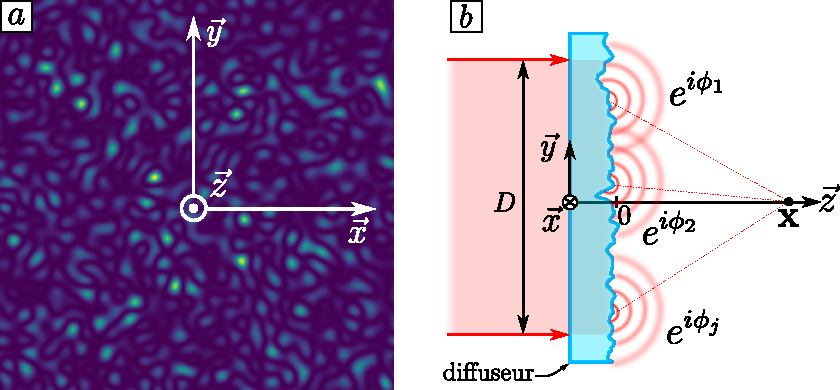
\includegraphics[width=0.9\textwidth]{Fig/Speckle/speckle_pattern.pdf}
\caption{\textbf{a: Génération d'une figure de speckle.} La diffraction d'une onde cohérente par une surface rugueuse appelée diffuseur résulte en l'interférence multiple d'une grand nombre d'ondes à déphasage aléatoire. La phase de chacune de ces ondes est déterminée par l'épaisseur de verre traversée en chaque point. \textbf{b: Motif de \speckle .} Un tel motif est composé de grains lumineux entourés de zones d'ombre, où l'intensité est quasiment nulle. }
\label{fig:speckle_pattern}
\end{figure}



\subsection{Statistiques de l'intensité d'un \speckle}
\label{sc:distribution_speckle}
Le phénomène de \speckle\ apparaît lorsque l'amplitude $E(\mathbf{x})$ au point d'observation $\mathbf{x}$ résulte de la somme d'un grand nombre N d'ondes indépendantes d'amplitude $E_0$ et de phases aléatoires $\phi_j$ comme illustré figure \ref{fig:speckle_pattern}.a. Cette amplitude peut alors s'écrire
\begin{equation}
E(\mathbf{x})=\sum_{j}^{N} E_0 e^{i \phi_j} \text{ .}
\end{equation}
En supposant qu'un grand nombre de grains du diffuseur participent à l'interférence au point d'observation ($\rdiff \ll D$ avec $\rdiff$ la taille typique d'un grain du diffuseur et $D$ la taille de l'éclairement incident), on peut appliquer le théorème central limite à l'amplitude rayonnée. En supposant de plus que les phases aléatoires $\phi_j$ sont réparties de manière homogène sur l'intervalle $\left[ 0,2\pi \right]$, les distributions de probabilités des parties réelle et imaginaire de l'amplitude sont données par la loi normale
\begin{equation}
\mathcal{P}(E_{\mathcal{R,I}})=\frac{1}{\sigma_E\sqrt{2\pi}} \exp{\left( -\frac{E_{\mathcal{R,I}}^2}{2 \sigma_E^2}\right) } \text{ ,}
\end{equation}
avec $E_{\mathcal{R}}$ et $E_{\mathcal{I}}$ les parties réelle et imaginaire du champ complexe $E=E_{\mathcal{R}} +i E_{\mathcal{I}}$ respectivement. Étant donné que les atomes ne sont sensibles qu'à l'intensité lumineuse $I=\left| E \right| ^2$, on montre alors que la distribution de probabilité de l'intensité lumineuse suit une loi exponentielle \citep{goodman2007speckle}
\begin{equation}
\mathcal{P}(I)=\frac{1}{\overline{I}}\exp{\left( -I/\overline{I} \right) } \text{ .}
\label{eq:proba_speckle}
\end{equation}
De manière générale, on appellera \emph{\speckle\ pleinement développé} tout \speckle\ vérifiant cette loi de probabilité. Deux conséquences importantes de cette loi sont à noter:
\begin{itemize}
\item[\textendash] L'écart-type $\sigma_I$ de la loi \ref{eq:proba_speckle} est égal à sa valeur moyenne $\overline{I}$, et donc le contraste $\sigma_I /\overline{I}$ d'une figure de \speckle\ pleinement développé est de 1. Une telle figure comportera alors des zones de forte intensité tout comme des zones d'intensité quasi-nulle. 
\item[\textendash] La probabilité d'obtenir une forte intensité lumineuse est exponentiellement petite, tandis que les zones de faible intensité sont beaucoup plus probables. Ainsi, une figure typique de \speckle\ (représentée figure \ref{fig:speckle_pattern}.b) est composée de maxima d'intensité lumineuse (\emph{grains de \speckle}) entourés de larges zones d'ombre.
\end{itemize}





\subsection{Propriétés du diffuseur}
\label{sc:prop_diffuseur}
L'analyse précédente décrivant la statistique de l'intensité lumineuse d'un \speckle\ pleinement développé repose sur deux hypothèses: 
\begin{itemize}
\item[\textendash] Il faut qu'un grand nombre d'émetteurs participe à l'interférence au point d'observation. Notamment, cela signifie que le diffuseur comporte un nombre suffisamment grand de \emph{grains} ($\rdiff \ll D$)  et que ceux-ci rayonnent au point d'observation. Ce dernier point sera illustré section \ref{sc:speckle_correlation}.
\item[\textendash] Pour que la distribution de probabilité de l'amplitude soit centrée en 0, propriété essentielle pour un \speckle\ pleinement développé, il faut que la distribution de phases soit suffisamment large de telle sorte que celle-ci puisse être considérée homogène sur l'intervalle $\left[ 0,2\pi \right]$. Cette condition de diffuseur fort se traduit en terme d'écart-type de la distribution de phases $\sigma_\phi \gg 2\pi$. 
\end{itemize}
Les deux grandeurs apparaissant dans ces hypothèses, $\rdiff$ et $\sigma_\phi$, sont fixées par les propriétés du diffuseur, que nous nous attacherons à décrire dans cette partie.

Dans le cadre de notre expérience, la génération du \speckle\ se fait par transmission d'une onde laser au travers d'une lame de verre dépolie, d'épaisseur locale $e(\mathbf{x}_0)$ aléatoire et répartie selon une distribution gaussienne de largeur $\sigmae$ et de valeur moyenne $\overline{e}$, où $\overline{\:\cdots\:}$ représente la moyenne sur les différentes réalisations de l'épaisseur aléatoire. On supposera que cette lame a été dépolie de manière homogène, ainsi, la statistique de l'épaisseur ne dépend pas de la position considérée sur la surface du diffuseur. On assimilera donc la distribution de l'épaisseur à un processus stationnaire. 

La phase localement accumulée par le faisceau laser incident lors de la traversée du diffuseur est proportionnelle à l'épaisseur traversée et donnée par
\begin{equation}
\phi(\mathbf{x}_0)=2\pi (n-1) \frac{e(\mathbf{x}_0)}{\lambda} \text{ ,}
\end{equation}
avec $n$ l'indice du verre et $\lambda\approx \SI{780}{\nano\metre}$ la longueur d'onde de l'onde laser. L'influence de cette phase sur l'amplitude du champ laser se traduit via la transmission locale du diffuseur
\begin{equation}
\tdiff(\mathbf{x}_0)=e^{i\phi(\mathbf{x}_0)}
\end{equation}
dont la valeur moyenne $\overline{\tdiff}$ caractérise le pouvoir diffusant. Pour une lame peu rugueuse, le faisceau est en moyenne peu affecté lors de sa traversée et l'on a $\overline{\tdiff}\approx 1$, tandis que dans le cas d'un diffuseur fort $\overline{\tdiff} \approx 0$. En fixant la phase moyenne $\overline{\phi}=0$, on montre annexe \ref{ch:anex_speckle} que \citep{denechaud2018vers}
\begin{equation}
\overline{\tdiff}=e^{-\frac{\sigma_{\phi}^2}{2}} \quad \text{avec} \quad \sigma_\phi=2\pi (n-1) \frac{\sigmae}{\lambda} \text{ .}
\label{eq:sigma_phi}
\end{equation}
Dans le cas d'un diffuseur de grande rugosité, dont l'épaisseur typique des grains $\sigmae$ est de l'ordre de plusieurs $\lambda$, on a $\sigma_\phi \gg 2\pi$ et cela permet donc de considérer que la distribution de phases est constante sur l'intervalle $\left[0,2\pi \right]$, essentiel pour un \speckle\ pleinement développé.

\begin{figure}
\centering
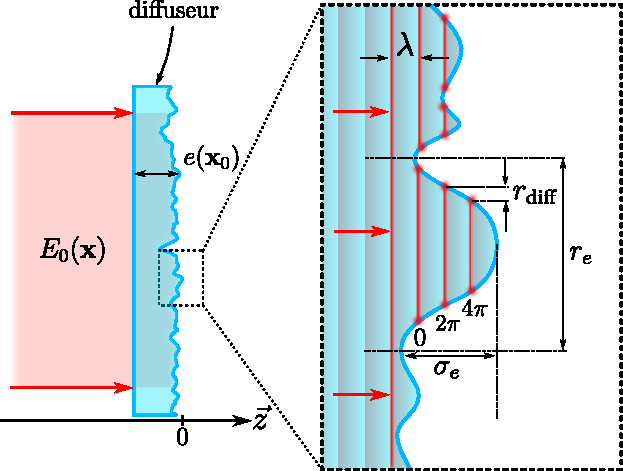
\includegraphics[scale=1]{Fig/Speckle/diffus_prop.pdf}
\caption{\textbf{Caractéristiques du diffuseur.} L'épaisseur aléatoire est caractérisée par une hauteur typique $\sigmae$ et une granularité de taille $r_e$. Pour $\sigmae \gg \lambda$, on a plusieurs oscillations de l'onde incidente dans le même grain, et donc $\tdiff$ qui est une fonction $2\pi-$périodique, voit sa corrélation réduite.}
\label{fig:diffus_prop}
\end{figure}

Les grains du diffuseur sont de plus caractérisés par une certaine extension spatiale typique $r_e$ correspondant à une largeur de corrélation de l'épaisseur. Celle-ci induit donc une corrélation spatiale de la transmission, décrite à l'aide la fonction de corrélation
\begin{equation}
\Cdiff(\mathbf{x}_0,\mathbf{x}'_0)=\overline{\tdiff(\mathbf{x}_0)\tdiff^*(\mathbf{x}'_0)}=\overline{e^{i(\phi(\mathbf{x}_0)-\phi(\mathbf{x}'_0))}} { .}
\label{eq:correlation_diffuseur}
\end{equation}

Puisque l'épaisseur et la phase sont proportionnelles, ces deux grandeurs sont corrélées sur la même taille $r_e$ correspondant à la granularité de la surface du verre. En revanche, dans le cas où $\sigmae \gg \lambda$ (ce qui est le cas sur notre expérience), l'onde oscille plusieurs fois dans le même grain du diffuseur. La transmission étant une fonction $2\pi-$périodique de la phase, celle-ci perd alors sa corrélation sur une taille $\rdiff \ll r_e$, voir figure \ref{fig:diffus_prop}. On montre alors annexe \ref{ch:anex_speckle} que la corrélation de la transmission à courte portée\footnote{La corrélation de la transmission tend suffisamment vite vers 0 pour que l'on puisse considérer que $\left|\mathbf{x}_0-\mathbf{x}'_0 \right| \ll r_e$ dans le cas où $\sigma_\phi \gg 2\pi$.} est de forme gaussienne:
\begin{equation}
\Cdiff(\mathbf{x}_0,\mathbf{x}'_0)\approx \exp{\left( -\frac{\left| \mathbf{x}_0 - \mathbf{x}'_0 \right| ^2}{2 \rdiff^2}\right) } \quad \text{avec} \quad \rdiff=r_e/\sigma_\phi \text{ .}
\end{equation}
$\rdiff$ joue alors le rôle de la taille effective d'un émetteur indépendant tel que considéré dans la section \ref{sc:distribution_speckle}. La condition d'un grand nombre d'émetteurs s'écrit alors $\rdiff \ll D$.

Enfin, il est possible de définir l'angle de diffusion $\theta_{\mathrm{diff}}=\lambda/\pi \rdiff=2(n-1) \sigmae/r_e$, qui est indépendant de la longueur d'onde de l'onde laser incidente. $\theta_{\mathrm{diff}}$ est donc une constante du diffuseur, fixée par les paramètres géométriques de celui-ci.










\subsection{Implémentation expérimentale}
\label{sc:montage_diffuseur}
Les expériences menées sur notre dispositif jusqu'en 2014 utilisaient un \speckle\ réalisé à la longueur d'onde de \SI{532}{\nano\metre}. Ce grand désaccord vers le bleu par rapport à la transition $\mathrm{D}_2$ du \isotope[87]{Rb} permet ainsi de s'affranchir de l'émission spontanée, même pour les très longs temps de propagation nécessaires à l'étude de la localisation d'Anderson. Depuis 2015 en revanche, l'équipe utilise un \speckle\ accordable autour de \SI{780}{\nano\metre} offrant ainsi la possibilité de réaliser un désordre attractif ou répulsif. Nous verrons section \ref{sc:potentiel_speckle} que cette accordabilité autour de la transition $\mathrm{D}_2$ offre un grand nombre de possibilités expérimentales, telles que la génération d'un désordre dépendant du spin.

\paragraph*{Mise en forme du faisceau \speckle}

\begin{figure}
\centering
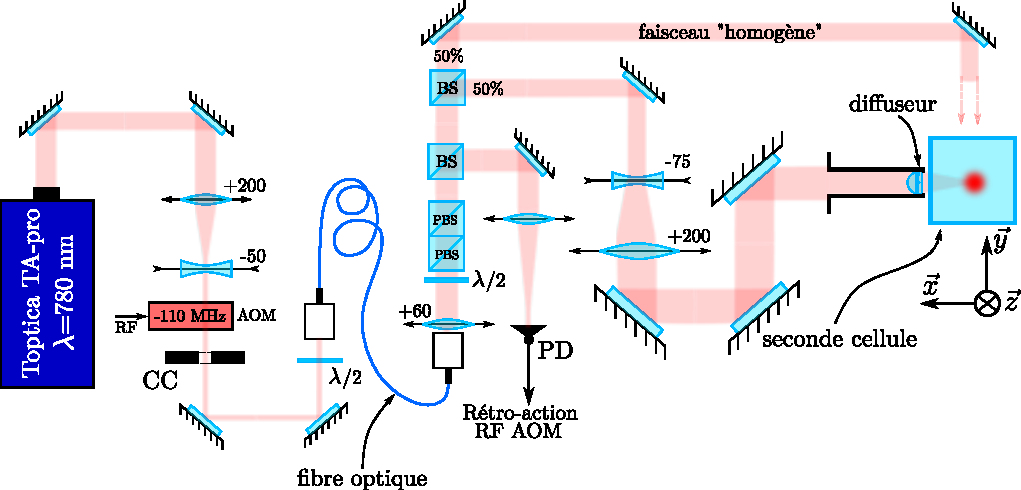
\includegraphics[width=\textwidth]{Fig/Speckle/montage_speckle_taus.pdf}
\caption{\textbf{Montage de génération du désordre optique.} Ce montage se décompose en deux parties, la première étant dédiée à la mise en forme du faisceau (cadre de gauche). Celui-ci est émis d'un laser Toptica TA-Pro, dont le mode et la polarisation sont filtrés, et la puissance est stabilisée. Dans un second temps, ce faisceau est focalisé sur les atomes et passe au travers du diffuseur générant le \speckle\ (cadre de droite).}
\label{fig:montage_speckle_taus}
\end{figure}

Par vœux de concision, seules les grandes lignes du montage de génération du \speckle\ à \SI{780}{\nano\metre} seront données ici, de nombreux détails à propos de ce montage pouvant être retrouvés dans les thèses de Jérémie Richard, Vincent Denechaud et Musawwadah Mukhtar \citep{denechaud2018vers, mukhtar2019state, richard2015propagation}. De plus, les détails des éléments du montage dépendent fortement de la mesure souhaitée comme nous le verrons dans la suite de chapitre, néanmoins la philosophie en reste inchangée.

Ce montage se décompose en deux parties, la première permettant de mettre en forme les propriétés du faisceau laser, et la seconde génère le désordre sur les atomes.

Le faisceau source du \speckle\ est émis par un laser industriel \emph{Toptica TA-Pro} \SI{2}{\watt} accordable autour de \SI{780}{\nano\metre}. Étant donné la proximité de la transition atomique, ce laser peut être asservi par battements sur le laser repompeur \emph{L2}\footnote{Le choix d'asservir ou non ce laser dépend du désaccord utilisé. Ainsi, nous verrons que le laser \speckle\ n'était pas asservi en fréquence pour la mesure du temps de diffusion élastique ($\left|\Delta\right|/2\pi\sim\SI{1}{\tera\hertz}$), tandis que ce fut le cas lors de la mesure des fonctions spectrales ($\left|\Delta\right|/2\pi\sim\SI{70}{\mega\hertz}$).}, ce qui permet alors d'en fixer la fréquence avec une précision de \SI{1}{\mega\hertz}. Le mode spatial et la polarisation du faisceau sont filtrés à l'aide d'une fibre optique à maintien de polarisation et de cubes séparateurs de polarisation. 

Une partie de la puissance du faisceau est ensuite prélevée et mesurée à l'aide d'une photodiode, et la rétroaction sur le faisceau à l'aide d'un modulateur acousto-optique (AOM pour l'anglais \emph{Acousto-Optic Modulator}) permet alors d'en stabiliser la puissance. La photodiode étant placée après la fibre optique et les cubes séparateurs de polarisation, la boucle d'asservissement de puissance permet de plus de s'affranchir des fluctuations de puissance dues à la polarisation et aux fluctuations du couplage. 

Enfin, le faisceau est séparé en deux parties par une séparatrice $50/50$, chacune de ces parties pouvant être envoyée sur les atomes. La partie réfléchie est ensuite agrandie à l'aide d'un télescope avant d'être focalisée sur les atomes et diffraction par le diffuseur, dont la géométrie sera présentée dans le paragraphe suivant. À ce stade, on dispose d'un faisceau de waist \SI{14.6}{\milli\metre} (rayon à $1/e^2$), de polarisation $\pi$ et dont la puissance est stabilisée et contrôlable.

Historiquement, la partie transmise était utilisée afin de réaliser une superposition cohérente de deux faisceaux \speckle , permettant d'obtenir un désordre isotrope\footnote{Comme nous le verrons section \ref{sc:correlation_longitudinale}, les grains d'un \speckle\ unique sont étendus suivant la direction longitudinale. L'interférence entre deux \speckles\ croisés permet de fortement réduite cette anisotropie \citep{piraud2012localisation}.} \citep{jendrzejewski2012quantum}. Aujourd'hui, ce faisceau est utilisé sans diffuseur et permet de réaliser un potentiel homogène servant à calibrer l'amplitude du potentiel.




%La spécificité de ce montage réside dans sa capacité à stabiliser par asservissement une très faible puissance optique, typiquement de quelques \SI{}{\micro\watt} compte-tenu de la proximité de la transition. Pour cela, 90\% de la puissance optique sont déviés vers une photodiode, dont la mesure permet de rétroagir sur la puissance du faisceau à l'aide d'un modulateur acousto-optique. Cette mesure à haute puissance permet de plus d'être particulièrement sensible aux fluctuations de puissance. 





\paragraph*{Génération du \speckle}

\begin{figure}
\centering
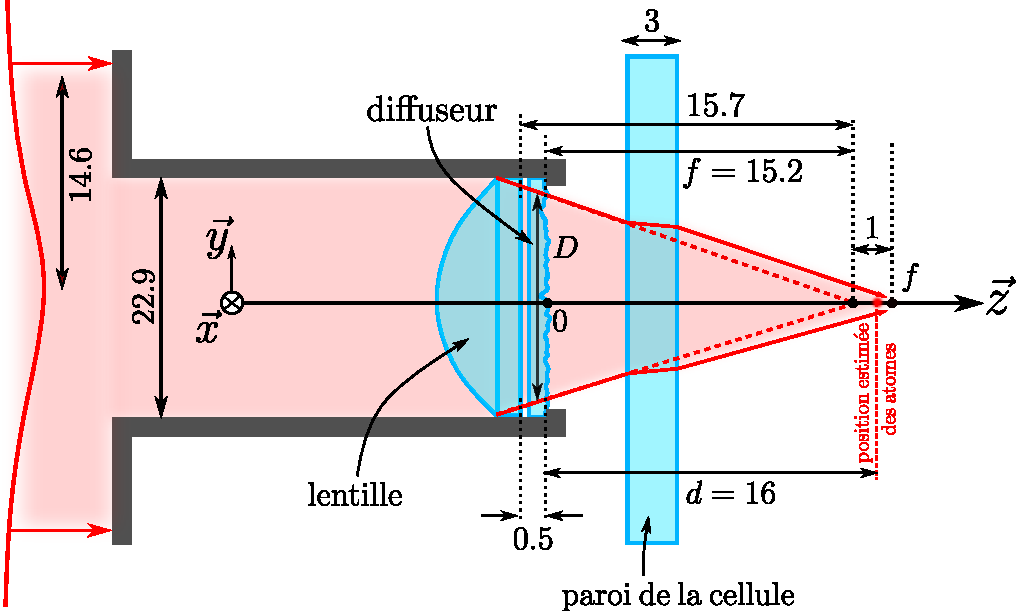
\includegraphics[width=0.9\textwidth]{Fig/Speckle/montage_diffuseur.pdf}
\caption{\textbf{Géométrie du montage de génération du \speckle .} Un faisceau gaussien incident de waist \SI{14.6}{\milli\metre} est tronqué dans un diaphragme de diamètre \SI{22.9}{\milli\metre} qui supporte le diffuseur. Ce faisceau est ensuite focalisé par une lentille asphérique épaisse de focale \SI{16}{\milli\metre} et traverse le diffuseur d'épaisseur \SI{0.5}{\milli\metre}. Le plan de focalisation est déplacé d'environ \SI{1}{\milli\metre} à cause de la paroi de la cellule à vide, d'épaisseur \SI{3}{\milli\metre}. Le plan repéré en rouge, correspondant à la surface moyenne du diffuseur, servira de plan de référence dans le cadre d'une géométrie effective illustrée figure \ref{fig:geometrie_effective_speckle}.}
\label{fig:montage_diffuseur}
\end{figure}

La génération du \speckle\ se fait selon le montage représenté figure \ref{fig:montage_diffuseur}. Un faisceau gaussien collimaté de waist \SI{14.6}{\milli\metre} et de longueur d'onde $\lambda=\SI{780}{\nano\metre}$, dont la mise en forme a été présentée dans le paragraphe précédent, est tronqué par un diaphragme de diamètre \SI{22.9}{\milli\metre}. Ce faisceau passe ensuite au travers d'une lentille asphérique épaisse (\textit{Thorlabs ACL2520-B}) de focale \SI{16.0}{\milli\metre} (et de frontale \SI{15.7}{\milli\metre}) montée dans ce même diaphragme. Le rôle de celle-ci est de focaliser la lumière sur les atomes\footnote{Nous verrons dans la section suivante que cela permet d'obtenir des grains de \speckle\ les plus petits possibles. En effet, on attend la manifestation d'effets quantiques sur la propagation d'une onde de matière dans un \speckle\ pour des longueurs d'onde de de Broglie plus grandes que la taille des grains de \speckle .}. Accolé à cette lentille se trouve un diffuseur \textit{Newport FSD10-3} possédant une épaisseur de \SI{0.5}{\milli\metre}\footnote{Cette épaisseur était initialement de \SI{3}{\milli\metre} avant d'être réduite à \SI{0.5}{\milli\metre} par l'atelier d'optique de l'IOGS.} et un angle de diffusion $\theta_{\mathrm{diff}}\approx\SI{5}{\degree}$. 

Enfin, ce faisceau convergent traverse la paroi de la cellule en verre sous ultra-vide d'épaisseur $e=\SI{3.0}{\milli\metre}$ et située à \SI{0.5}{\milli\metre} de la monture du diffuseur. Le matériau de cette cellule est du Vycor, d'indice optique $n=1.46$. L'épaisseur de cette cellule, considérée comme une lame à faces parallèles, induit un décalage des rayons lumineux par réfraction, décalage représenté figure \ref{fig:montage_diffuseur} montrant la trajectoire des rayons lumineux en absence de la paroi par des traits pointillés. La présence de la paroi entraîne donc un déplacement du plan de focalisation donné par $\Delta d=e(1-1/n)\approx \SI{1}{\milli\metre}$. La distance focale en présence de la paroi de la cellule est alors de \SI{17.0}{\milli\metre}.


En choisissant pour origine de l'axe $\vec{z}$\footnote{L'axe $\vec{z}$ utilisé dans ce chapitre correspond à la direction de propagation du faisceau \speckle . Dans le repère de l'expérience, il s'agit en réalité de l'axe $\vec{x}$, perpendiculaire au plan formé par les faisceaux du piège optique.} la surface du diffuseur, la position du plan de focalisation se trouve à $f=\SI{16.2}{\milli\metre}$. Dans ce repère, la position des atomes dans le piège optique est estimée quant à elle a $d=16\pm\SI{0.5}{\milli\metre}$, dont la valeur est proche de celle de la position du plan de focalisation. Néanmoins, l'incertitude liée à la position des atomes est cruciale, celle-ci pouvant conduire à un écart de \SI{0.7}{\milli\metre} du plan de focalisation. Il est ainsi primordial de connaître les propriétés du \speckle\ autour du plan de focalisation. 


\paragraph*{Géométrie effective du montage du diffuseur}
La lentille asphérique utilisée pour la focalisation du faisceau sur les atomes étant épaisse\footnote{L'épaisseur au centre est de \SI{12}{\milli\metre} pour une frontale de \SI{15.7}{\milli\metre}.}, le faisceau est donc fortement affecté par sa traversée. L'éclairement dans le plan du diffuseur correspond donc à l'éclairement incident gaussien de waist \SI{14.6}{\milli\metre} (rayon à $1/e^2$) tronqué par une pupille de diamètre \SI{22.9}{\milli\metre} et ayant déjà subi un effet de focalisation. Il a été déterminé par photographie que le profil de l'éclairement dans le plan du diffuseur est aussi de forme gaussienne tronquée, avec un waist $w_0=9\pm\SI{1}{\milli\metre}$ et une pupille de diamètre $D=20.3\pm\SI{0.1}{\milli\metre}$.

Il est alors possible de décrire le montage du diffuseur et le champ incident à l'aide d'une géométrie effective simplifiée illustrée figure \ref{fig:geometrie_effective_speckle}. On considèrera ainsi que le profil d'intensité au niveau du diffuseur est donné par une forme gaussienne de largeur $w=9\pm\SI{1}{\milli\metre}$ tronquée par une diaphragme de diamètre $D=20.3\pm\SI{0.1}{\milli\metre}$ et convergeant à la distance $f=\SI{15.2}{\milli\metre}$\footnote{Si la présence de la paroi de la cellule entraîne un déplacement du plan focalisation, celle-ci ne modifie pas l'ouverture numérique du système, c'est à dire l'angle des rayons avec l'axe optique. Comme nous le verrons dans la suite, il s'agit de la quantité qui décrit, avec la longueur d'onde, les propriétés spatiales d'un champ de \speckle .}. Ceci entraîne une ouverture numérique maximale $\ON=\sin{(\theta_{\mathrm{max}})}=0.55\pm0.02$. Dans le cadre de cette géométrie effective, la position des atomes est estimée à $d=15\pm\SI{0.5}{\milli\metre}$.

\begin{figure}
\centering
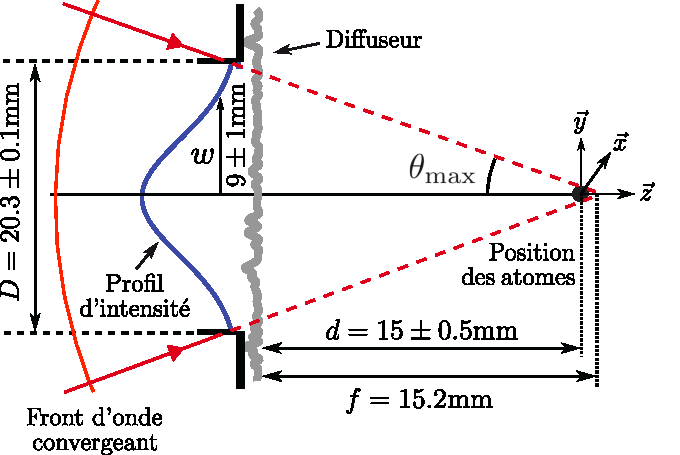
\includegraphics[scale=0.9]{Fig/Speckle/geometrie_effective_speckle.pdf}
\caption{\textbf{Géométrie effective du montage du diffuseur.} L'épaisseur de la lentille n'étant pas négligeable, l'éclairement au niveau du diffuseur a déjà subi un effet de focalisation comparé à celui au niveau de la lentille. Cela se traduit par un front d'onde au niveau du diffuseur qui est convergeant, avec un profil gaussien de largeur $w\approx\SI{9}{\milli\metre}$ tronqué à un diamètre $D\approx\SI{20.3}{\milli\metre}$.}
\label{fig:geometrie_effective_speckle}
\end{figure}


\paragraph*{Amplitude rayonnée}
L'utilisation de ce modèle à géométrie effective permet de décrire simplement les propriétés du champ de \speckle . En particulier, l'amplitude rayonnée $E(\xd)$ est simplement donnée par le principe de Huygens-Fresnel\footnote{Nous utilisons ici l'approximation paraxiale (voir annexe \ref{ch:anex_speckle}), dont la pertinence sera discutée à postériori.}:
\begin{equation}
E(\xd) \propto \int{\mathrm{d}\xzero \: \Ediff (\xzero) \exp{\left( ik\frac{\xzero^2}{2\deff} \right) } \: \exp{\left( -ik \frac{\xd \cdot \xzero}{d} \right) } } \text{ ,}
\label{eq:amplitude_rayonnee}
\end{equation}
où l'ensemble des points $\lbrace\xd\rbrace$ correspond au plan $\lbrace x,y,z=d \rbrace$ situé à une distance $d$ de la surface du diffuseur. L'ensemble des points $\lbrace\xzero\rbrace$ décrit le plan du diffuseur $\lbrace x,y,z=0 \rbrace$, $k=2\pi/\lambda$ est le nombre d'onde et $\deff$ correspond à une distance effective donnée par $1/\deff=1/d-1/f$.

$\Ediff (\xzero)$ correspond à l'amplitude dans le plan de référence du diffuseur, qu'il est possible de décomposer sous la forme 
\begin{equation}
\Ediff(\xzero)=\Ezero(\xzero) \tdiff(\xzero) \quad \text{avec} \quad \Ezero(\xzero) = E_\mathrm{inc} (\xzero) m(\xzero) \text{ ,}
\end{equation}
où $\tdiff(\xzero)$ est la transmission du diffuseur, $E_{\mathrm{inc}}(\xzero)$ est le champ incident\footnote{Il s'agit du faisceau gaussien de waist \SI{9}{\milli\metre} dans notre géométrie effective.}, et $m(\xzero)=\Theta(\left| \xzero \right| - D/2)$ avec $\Theta$ la fonction de Heaviside est un masque représentant le diaphragme de diamètre $D$. $\Ezero(\xzero)$ correspond alors au champ au niveau du diffuseur, de forme gaussienne tronquée et convergente.


\section{Propriétés spatiales d'un champ de \speckle}
\label{sc:speckle_correlation}

Le \speckle\ résultant de la propagation d'un faisceau transmis par le diffuseur, il est donc régit par les lois de la diffraction. Il est donc possible de déduire les propriétés spatiales du \speckle\ de celles du diffuseur ainsi que de celles de l'éclairement incident. Notamment, les variations spatiales du champ de \speckle\ sont décrites quantitativement par sa fonction de corrélation, dont l'étude permet de déterminer toutes les tailles caractéristiques d'intérêt pour notre expérience. Parmi celles-ci, nous nous concentrerons sur l'extension du champ de \speckle\ ainsi que sur les tailles moyennes des grains de lumière. 

Dans cette section, nous allons nous attacher à décrire ces échelles de longueur caractéristiques autour du plan de focalisation à l'aide de la fonction de corrélation du champ de \speckle\ et de son intensité moyenne, dont le détail des calculs est donné en annexe \ref{ch:anex_speckle}. 

De plus, lors de la conception de ce système, l'extension du champ de \speckle\ ainsi que les tailles des grains de \speckle\ ont été mesurées expérimentalement sur un montage reproduisant exactement les conditions réelles en présence de la cellule à vide, celle-ci empêchant de faire des mesures in-situ. La description de ces mesures et de leur traitement sont référencées dans la thèse de Jérémie Richard \citep{richard2015propagation}.




\subsection{Extension transverse du champ de speckle le long le l'axe optique}
%%%%%%%%%%%%%%%%%%%%%%%%%%%%%%%%%%%%%%%%
\begin{comment}
Afin de déterminer l'extension transverse du champ de \speckle , il est nécessaire de calculer le profil d'intensité moyenne $\overline{I}(\xd)$, où l'ensemble des points $\lbrace\xd\rbrace$ correspond au plan $\lbrace x,y,z=d \rbrace$ situé à une distance $d$ de la surface du diffuseur. Pour cela, explicitons le champ rayonné $E(\xd)$ à l'aide du principe de Huygens-Fresnel dans l'approximation paraxiale:
\begin{equation}
E(\xd) \propto \int{\mathrm{d}\xzero \: \Ediff (\xzero) \exp{\left( ik\frac{\xzero^2}{2\deff} \right) } \: \exp{\left( -ik \frac{\xd \cdot \xzero}{d} \right) } } \text{ ,}
\label{eq:amplitude_rayonnee}
\end{equation}
où $k=2\pi/\lambda$ est le nombre d'onde et $\deff$ correspond à une distance effective donnée par $1/\deff=1/d-1/f$. L'ensemble des points $\lbrace\xzero\rbrace$ décrit le plan du diffuseur $\lbrace x,y,z=0 \rbrace$, et $\Ediff (\xzero)$ correspond au champ dans ce plan, qu'il est possible de décomposer sous la forme 
\begin{equation}
\Ediff(\xzero)=\Ezero(\xzero) \tdiff(\xzero) \quad \text{avec} \quad \Ezero(\xzero) = E_\mathrm{inc} (\xzero) m(\xzero) \text{ ,}
\end{equation}
où $\tdiff(\xzero)$ est la transmission du diffuseur, $E_{\mathrm{inc}}(\xzero)$ est le champ incident\footnote{Il s'agit du faisceau gaussien de waist \SI{9}{\milli\metre} dans notre géométrie effective.}, et $m(\xzero)=\Theta(\left| \xzero \right| - D/2)$ avec $\Theta$ la fonction de Heaviside est un masque représentant le diaphragme de diamètre $D$. $\Ezero(\xzero)$ correspond alors au champ au niveau du diffuseur, et on supposera dans la suite que celui-ci varie lentement à l'échelle des variations de $\tdiff(\xzero)$, c'est à dire que $\Ezero(\xzero+\delta\xzero)\approx\Ezero(\xzero)$ avec $\delta\xzero$ de l'ordre de $\rdiff$.
\end{comment}
%%%%%%%%%%%%%%%%%%%%%%%%%%%%%%%%%%%%%%%%%%%%%%%%

Afin de déterminer l'extension transverse du champ de \speckle , il est nécessaire de calculer le profil d'intensité moyenne $\overline{I}(\xd)$ à partir de l'expression de l'amplitude rayonnée \ref{eq:amplitude_rayonnee}. En remarquant que le champ $\Ezero(\xzero)$ varie lentement à l'échelle des variations de $\tdiff(\xzero)$, on peut écrire que $\Ezero(\xzero+\delta\xzero)\approx\Ezero(\xzero)$ avec $\delta\xzero$ de l'ordre de $\rdiff$. 

On montre alors (voir annexe \ref{ch:anex_speckle}) que le profil d'intensité moyenne à la distance $d$ peut s'écrire \citep{gatti2008three}
\begin{align}
\nonumber\overline{I}(\xd)&=\overline{E(\xd) E^*(\xd)} \\
&\propto I_0 \left( \frac{\deff}{d} \xd \right) \ast \widetilde{\Cdiff}\left( \frac{\xd}{\lambda d} \right) \text{ ,}
\label{eq:evolution_extension_transverse_speckle}
\end{align}
où le symbole $\ast$ dénote le produit de convolution. L'évolution du profil d'intensité moyenne en fonction de la distance $d$ est alors dû à deux contributions dont l'interprétation physique est la suivante:
\begin{itemize}
\item[\textendash] Le premier terme correspond à l'effet de la lentille dans le cadre de l'optique géométrique, et focalise donc le profil d'intensité initiale $I_0(\xzero)=\left| \Ezero(\xzero) \right|^2$ dans le plan focal $\lbrace x,y,z=f\rbrace$. Cette focalisation se traduit au travers d'un changement d'échelle de l'intensité par le facteur $d/\deff=\left| d-f \right| /f$. Ainsi, la taille de ce faisceau focalisé décroît avec la distance jusqu'à s'annuler dans le plan focal, comme prédit par l'optique géométrique.
\item[\textendash] Le second terme est la transformée de Fourier de la fonction de corrélation du diffuseur $\Cdiff(\xzero)$. Ce terme traduit la diffraction de l'onde incidente par les grains du diffuseur de taille $\rdiff$. À partir de l'expression \ref{eq:correlation_diffuseur} de $\Cdiff(\xzero)$, on trouve que ce terme correspond à une gaussienne dont la largeur est donnée par $\lambda d/ \pi \rdiff$, qui croît linéairement avec la distance $d$.
\end{itemize}
Ces dépendances sont illustrées figure \ref{fig:speckle_extension}, où le fond rose correspond au premier terme de focalisation, tandis le fond orange illustre le second terme de diffraction issu du centre du diffuseur. On identifie alors deux régimes pour lesquels un terme est prépondérant. 

\begin{figure}
\centering
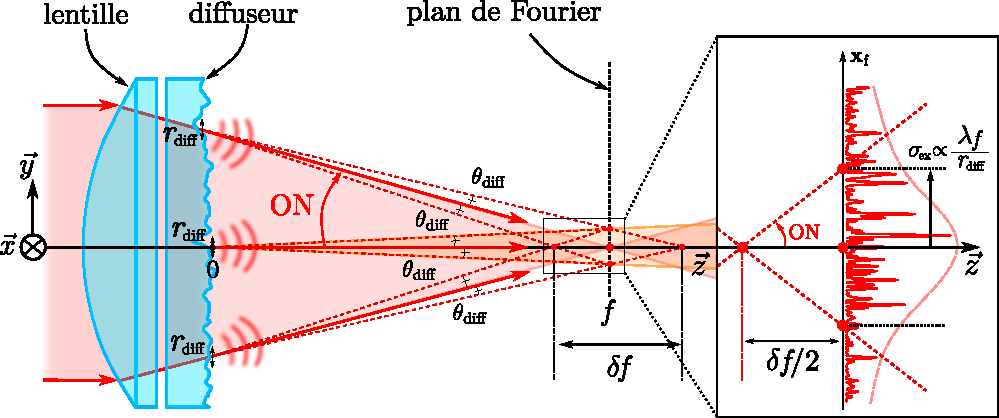
\includegraphics[width=\textwidth]{Fig/Speckle/speckle_extension.pdf}
\caption{\textbf{Extension du champ de speckle.} L'extension du faisceau de speckle est due à deux effets distincts, la focalisation du faisceau incident et la diffraction du faisceau par le diffuseur suivant un angle $\theta_{\mathrm{diff}}$. La contribution de la focalisation à l'extension du faisceau est illustrée par des flèches rouges et un remplissage rose, tandis que celle de la diffraction correspond à un remplissage orange. La région aux alentours du plan focal est particulièrement intéressante car il s'agit de celle où l'ensemble des émetteurs contribuent à l'éclairement, chaque émetteur diffractant dans un cône d'angle $\theta_{\mathrm{diff}}$ illustré par des pointillés rouges. Dans le cas où l'angle de diffusion est petit devant l'ouverture numérique $\theta_{\mathrm{diff}} \ll \ON$, on peut estimer par trigonométrie l'étendue de cette région à $\delta f/2= \speckleext / \ON$ (encart).}
\label{fig:speckle_extension}
\end{figure}

Dans une première région, loin du plan focal de la lentille, la taille du faisceau est donnée par l'effet de focalisation de la lentille. Une seconde région, proche du plan focal de la lentille, est dominée par l'effet de diffraction des émetteurs du diffuseur, la taille de l'éclairement incident étant fortement réduite par focalisation. Ainsi, pour une zone très proche du plan focal de la lentille, on peut décrire le profil d'intensité lumineuse par 
\begin{equation}
\overline{I}\propto \mathrm{TF} \left[ \Cdiff \right] (\xf/\lambda f)
\end{equation}
où l'ensemble des points $\lbrace \xf \rbrace$ correspond au plan de Fourier\footnote{Dans le plan focal $\lbrace x,y,z=f\rbrace$, le champ rayonné est alors la transformée de Fourier du champ incident comme illustré par la formule \ref{eq:amplitude_rayonnee}. Il s'agit d'une propriété bien connue des lentilles de pouvoir ramener l'infini de la diffraction de Fraunhofer à distance finie.} $\lbrace x,y,z=f \rbrace$, et $\Cdiff$ est la fonction de corrélation du diffuseur, de forme de gaussienne avec une largeur $\rdiff$. Le profil d'intensité lumineuse dans le plan de Fourier est alors donné par 
\begin{equation}
\overline{I}(\xf)\propto \exp{(-\frac{2 \left| \xf \right|^2}{\speckleext})} \quad \text{avec} \quad \speckleext = \frac{\lambda f}{\pi \rdiff} \text{ .}
\label{eq:intensite_moyenne_speckle}
\end{equation}
$\speckleext$ correspond donc au waist du profil d'intensité moyenne, dont l'expression peut se réécrire à l'aide de l'angle du diffusion $\speckleext=\theta_{\mathrm{diff}} f = 1.5\pm\SI{0.1}{\milli\metre}$. Donc, dans le plan de Fourier, l'extension du champ de \speckle\ ne provient que de l'effet de la diffraction des émetteurs individuels dont les faisceaux se recouvrent tous, comme illustré figure \ref{fig:speckle_extension} par la zone orange.

Cette condition de recouvrement des faisceaux provenant de l'ensemble des émetteurs du diffuseur permet de considérer que dans cette région le \speckle\ est entièrement développé. Afin d'en déterminer l'étendue longitudinale, on s'intéresse aux positions de l'espace où l'ensemble des faisceaux provenant du diffuseur participent. Dans la limite $\theta_{\mathrm{diff}} \ll \ON$, on détermine par trigonométrie que cette zone s'étend de part et d'autre du plan de Fourier sur une distance $\delta f/2\approx \speckleext /\ON =2.5\pm\SI{0.1}{\milli\metre}$ (voir figure \ref{fig:speckle_extension}), délimitant ainsi les régions décrites précédemment. Par analogie avec un faisceau gaussien, on appellera $\delta f$ la \emph{distance de Rayleigh} du champ de \speckle , et sa valeur nous assure que les atomes se trouveront dans la zone où le \speckle\ est pleinement développé, celle-ci étant un ordre de grandeur plus grande que l'incertitude de positionnement des atomes.















\subsection{Longueur de corrélation transverse le long de l'axe optique}
\label{sc:correlation_transverse}
La seconde taille caractéristique du \speckle , la taille des grains de lumière, est une grandeur d'une importance capitale pour la physique du désordre. Si l'extension du faisceau de \speckle\ est une grandeur d'intérêt pratique (celle-ci donne une borne supérieure sur les tailles de nuages et détermine le potentiel maximal accessible en fonction de la puissance du faisceau laser), nous verrons chapitre \ref{ch:TauS_PRL} que la taille des grains de \speckle\ influe sur la dynamique de la propagation d'une onde en milieu désordonné.

Le potentiel ressenti par les atomes étant proportionnel à l'intensité lumineuse, on peut définir la taille des grains du potentiel à l'aide de la fonction de corrélation en intensité du \speckle . En utilisant le théorème de Wick pour les variables aléatoires gaussiennes, il est possible de relier la fonction de corrélation en intensité à la fonction de corrélation en amplitude du \speckle :
\begin{equation}
\overline{I(\xd) I(\xd')}=\overline{I(\xd)}\;\overline{I(\xd')} + \left| \overline{E(\xd)E^*(\xd')} \right|^2 \text{ ,}
\label{eq:theoreme_wick}
\end{equation}
où les positions $\xd$ et $\xd'$ correspondent à deux points dans le plan $\lbrace x,y,z=d\rbrace$ transverse à l'axe optique. 

Dans les conditions expérimentales usuelles, il est possible de négliger l'effet de l'extension spatiale finie du \speckle , celle-ci étant très grande à l'échelle des grains de \speckle . Dans ce régime, on peut alors considérer que le premier terme de l'équation \ref{eq:theoreme_wick} est constant et égal à $\overline{I}^2$. On définit alors la taille des grains du potentiel à l'aide la fonction de corrélation des fluctuations d'intensité:
\begin{equation}
\overline{\delta I(\xd) \delta I(\xd')} = \left| \overline{E(\xd)E^*(\xd')} \right|^2 \text{ ,}
\end{equation}
où $\delta I(\xd)=I(\xd)-\overline{I}(\xd)$ correspond aux fluctuations statistiques d'intensité. 

À l'échelle des grains de \speckle , on peut considérer que la fonction de corrélation en amplitude ne dépend uniquement que de la différence des positions considérées. On montre annexe \ref{ch:anex_speckle} que la fonction de corrélation transverse en amplitude le long de l'axe optique peut s'écrire \citep{gatti2008three}:
\begin{align}
\nonumber \CE(\xd,\xd') &= \overline{E(\xd) E^*(\xd')} \\
& \propto \widetilde{I_0}\left( \frac{\delta\xd}{\lambda d}\right) \ast \Cdiff\left( \frac{\deff}{d} \delta \xd \right) \text{ ,}
\label{eq:correlation_transverse_speckle}
\end{align}
où $\delta\xd=\xd'-\xd$. De même que pour l'extension spatiale du champ de \speckle , la fonction de corrélation transverse résulte de deux contributions, dont les interprétations physiques sont les suivantes:
\begin{itemize}
\item[\textendash] Le premier terme correspond à la transformée de Fourier de l'intensité lumineuse dans le plan du diffuseur. Il s'agit ici du motif de diffraction à l'infini en l'absence du diffuseur, dont la taille est proportionnelle à la distance. Ce facteur d'échelle s'interprète comme une diminution de l'ouverture numérique au fur et à mesure de l'éloignement avec le diffuseur, comme indiqué par la relation $\ON'(d)=D/2d$ en considérant les rayons les plus inclinés, avec $D$ la taille du diaphragme de l'éclairement au niveau du diffuseur. Ce terme conduit donc à largeur de l'ordre de $\sim\lambda / \pi \ON'(d)$, qui croît linéairement avec la distance $d$. 
\item[\textendash] Le second terme décrit quant à lui le fait que les grains du diffuseur ne diffractent que selon un angle $\theta_{\mathrm{diff}}$. De fait, ce terme décrit les régions de l'espace dans lesquelles l'ensemble du diffuseur ne participe pas à l'interférence au point $\xd$, comme illustré par la zone orange figure \ref{fig:correlation_speckle}. Ce terme joue ainsi le rôle d'ouverture numérique effective, dont l'expression $\ON_{\mathrm{eff}}(d)=\theta_{\mathrm{diff}} f/\left| d-f \right|$ peut être obtenue par trigonométrie \citep{richard2015propagation}. L'écriture de ce terme donnée équation \ref{eq:correlation_transverse_speckle} permet néanmoins d'obtenir une expression simple de la largeur induite pour la fonction de corrélation transverse: $\sim\lambda /\pi \ON_{\mathrm{eff}} (d)$.
\end{itemize}
La largeur de la fonction de corrélation apparaît alors comme la plus petite taille permise par les lois de la diffraction: il s'agit de la limite de diffraction. L'étude de la taille transverse des grains de \speckle\ se résume alors à l'évolution de l'ouverture numérique le long de l'axe de propagation du faisceau.

\begin{figure}
\centering
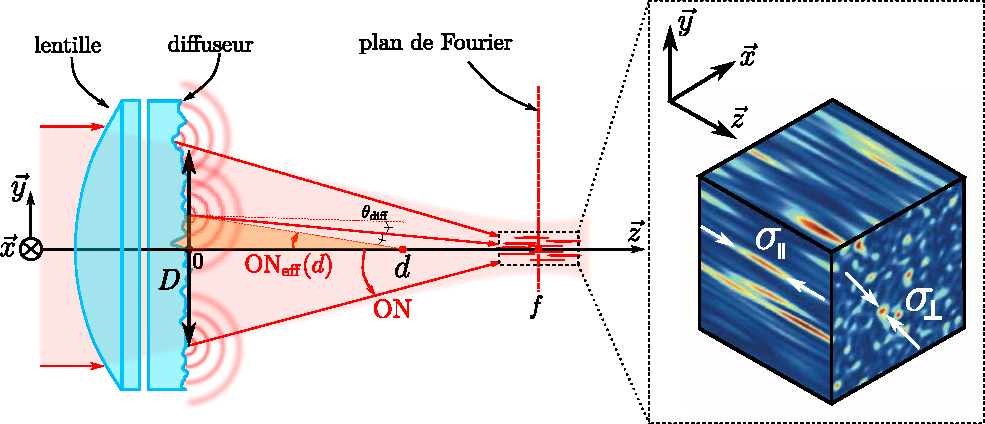
\includegraphics[width=\textwidth]{Fig/Speckle/correlation_speckle.pdf}
\caption{\textbf{Tailles des grains de speckle.} La taille transverse $\sigmap$ des grains de \speckle\ est donnée par la limite de diffraction, et dépend donc de l'ouverture numérique à la position d'observation $d$. Loin du plan de Fourier, seule une zone réduite du diffuseur participe à l'interférence, réduisant donc l'ouverture numérique (zone orangée). \textbf{Encart:} Simulation tridimensionnelle d'un champ de \speckle . Celle-ci fait apparaître une forme très allongée des grains selon la direction longitudinale. La taille longitudinale $\sigmal$ des grains est de l'ordre de la distance de Rayleigh associée à la taille transverse $\sigmap$ comme on le verra section \ref{sc:correlation_longitudinale}.}
\label{fig:correlation_speckle}
\end{figure}

À l'instar de l'extension du champ de \speckle , il est possible d'identifier deux régions dans lesquelles le comportement de la largeur de la fonction de corrélation transverse en amplitude du \speckle\ est majoritairement dû à l'un des effets mentionnés ci-dessus. La frontière entre ces deux régions est donnée, comme pour l'extension du \speckle , par la distance de Rayleigh $\delta f$ du champ lumineux qui caractérise, rappelons-le, l'étendue sur laquelle l'ensemble de diffuseur participe à l'amplitude rayonnée.

Nous considérerons donc dans la suite que les atomes se trouvent à proximité du plan de Fourier, et la fonction de corrélation sera dominée par le régime de diffraction à l'infini, où l'ouverture numérique y est maximale. La fonction de corrélation des fluctuations d'intensité s'écrit alors simplement
\begin{equation}
\overline{\delta I (\xf) \delta I (\xf + \delta \xf)} \propto \left| \mathrm{TF} \left[ I_0 \right] (\delta \xf / \lambda f \right| ^2 \text{ ,}
\end{equation}
qui n'est autre que le théorème de Van Cittert-Zernike en remarquant que la fonction de corrélation $\overline{\delta I(\xf)\delta I(\xf+\delta\xf)}$ correspond au degré de cohérence spatiale.
Dans la suite, nous assimilerons la forme de cette fonction de corrélation à une gaussienne (voir section \ref{sc:speckle_non_paraxial}), cependant, la forme exacte de la fonction de corrélation aux alentours du plan de Fourier nécessite tout de même une connaissance fine du profil d'intensité dans le plan du diffuseur\footnote{L'assimilation à une forme gaussienne revient à considérer que l'effet du diaphragme sur l'éclairement incident est négligeable. Cette simplification n'est valable que dans le cas de la corrélation transverse, l'effet du diaphragme étant bien plus marqué dans le cas de la corrélation longitudinale (voir sections \ref{sc:correlation_longitudinale} et \ref{sc:speckle_non_paraxial}).}. 

Nous retiendrons ici que la taille transverse des grains de lumière est donnée par la limite de diffraction du système, $\sigmap\sim \lambda/\pi\ON$ de l'ordre de \SI{0.5}{\micro\metre}, bien inférieure à l'extension du faisceau de \speckle\ $\sigmap \ll \speckleext$. Une calibration précise de la taille transverse des grains de \speckle\ est présentée section \ref{sc:speckle_non_paraxial}.




\subsection{Longueur de corrélation longitudinale autour du plan de Fourier}
\label{sc:correlation_longitudinale}
Comme représenté figure \ref{fig:correlation_speckle}, les grains de \speckle\ possèdent une extension longitudinale finie. De même que dans le cas de l'extension transverse des grains, la taille longitudinale des grains de \speckle\ est donnée par la largeur de la fonction de corrélation longitudinale des fluctuations des grains de \speckle\ aux alentours du plan de Fourier:
\begin{equation}
\overline{\delta I(f) \delta I( f + \delta z)}=\left| \overline{E(f) E^*(f+\delta z)} \right|^2 \text{ ,}
\label{eq:correlation_intensite_longitudinale}
\end{equation}
évaluée aux positions $\lbrace 0,0,z=f \rbrace$ et $\lbrace 0,0,z=f+\delta z \rbrace$ sur l'axe optique.

En supposant que l'extension longitudinale $\delta f$ du champ de \speckle\ soit très grande devant la taille longitudinale des grains, on peut se limiter à des petits déplacements $\delta z \ll \delta f$. On montre alors que la corrélation longitudinale en amplitude aux alentours du plan de Fourier peut s'écrire \citep{magatti2009three}:
\begin{equation}
\overline{E(f)E^*(f+\delta z)} \propto \int{\mathrm{d} \xzero I_0 (\xzero) e^{i\pi \xzero^2 \delta z / \lambda f^2} } \text{ .}
\label{eq:correlation_longitudinale_1_speckle}
\end{equation}

On retrouve ainsi un comportement similaire à celui de la corrélation transverse aux alentours du plan de Fourier: la fonction de corrélation ne dépend que de l'éclairement incident. Cependant, la détermination de la fonction de corrélation longitudinale est plus compliquée que celle de la corrélation transverse, celle-ci ne se résumant pas qu'à une simple transformation de Fourier. Avant de donner une expression analytique dans un cas précis, il possible de donner une estimation de la longueur de corrélation à l'aide de la \emph{méthode du col}. En effet, les valeurs de $\xzero$ qui contribuent significativement à l'intégrale sont celles pour lesquelles la phase $\pi \xzero^2 \delta z /\lambda f^2$ est très petite devant 1. On peut alors obtenir une estimation de la longueur de corrélation longitudinale:
\begin{equation}
\sigmal \sim \frac{\lambda }{ \pi \ON^2} \text{ .}
\label{eq:longueur_correlation_longitudinale}
\end{equation}
La taille longitudinale des grains apparaît alors comme étant la longueur de Rayleigh associée à la taille transverse des grains, ceux deux grandeurs étant reliées par $\sigmal \sim \sigmap /\ON$.







\paragraph*{Forme de la fonction de corrélation longitudinale}

Il est possible d'obtenir des expressions analytiques de la fonction de corrélation longitudinales pour certains profils d'intensité. Notamment, on peut montrer que dans le cas d'un éclairement purement gaussien, la fonction de corrélation \ref{eq:correlation_intensite_longitudinale} est de forme lorentzienne \citep{goodman2007speckle}:
\begin{equation}
\overline{\delta I(f) \delta I(f+\delta z)} \propto \frac{1}{1+4\delta z^2/\sigmal^2}
\end{equation}
avec $\sigmal=4\lambda f^2/\pi w^2$ et $w$ le waist du faisceau incident. On retrouve ainsi, à un facteur numérique près, la prédiction de la formule \ref{eq:longueur_correlation_longitudinale}. Un second cas d'intérêt correspond à celui d'un faisceau homogène tronqué par un diaphragme de diamètre $D$. Dans cette situation, la fonction de corrélation longitudinale \ref{eq:correlation_intensite_longitudinale} possède une forme en sinus cardinal au carré.

Dans le cas de notre éclairement à la fois gaussien et tronqué par un diaphragme, la fonction de corrélation possède donc une forme complexe proche d'une fonction lorentzienne et d'un sinus cardinal au carré, voir figure \ref{fig:speckle_correlations_exp}. Une calibration expérimentale de la longueur de corrélation longitudinale, donnée par la largeur de cette fonction de forme complexe, est présentée dans la section suivante.


















\subsection{Effets non-paraxiaux sur les corrélations du \speckle\ }
\label{sc:speckle_non_paraxial}

La forme des fonctions de corrélations étant directement donnée par celle de l'intensité $I_0(\xzero)$, la détermination précise des longueurs de corrélation du \speckle\ demande une connaissance fine de l'éclairement dans le plan du diffuseur. Cependant, les considérations sur l'éclairement au niveau du diffuseur présentées section \ref{sc:montage_diffuseur} ne suffisent pas à reproduire les fonctions de corrélations expérimentales (voir figure \ref{fig:speckle_correlations_exp}, courbes oranges), mesurées par le biais de corrélations d'images de \speckle\ obtenues à l'aide d'un objectif de microscope à haute résolution placé sur une platine de translation contrôlée électroniquement. Le procédé de mesure est décrit dans la thèse de Jérémie Richard \citep{richard2015propagation}. 

Cette différence observée s'explique par le fait que les expressions des fonctions de corrélation des fluctuations d'intensité ont été obtenues dans le cadre de l'approximation paraxiale. Si l'utilisation d'un système de grande ouverture numérique permet certes d'obtenir les tailles de grains les plus petites possible, cela remet en cause l'approximation paraxiale utilisée pour décrire les caractéristiques spatiales de notre champ de tavelures. En particulier, notre système permet d'obtenir une grande ouverture numérique $\ON=\sin{\theta_{\mathrm{max}}}=0.55\pm 0.02$ et cela implique que certains rayons lumineux sont inclinés d'un angle de plus de \SI{30}{\degree} par rapport à l'axe optique, pour lesquels l'approximation $\sin{\theta}=\theta$ n'est plus suffisante.

Notons tout de même que la forme de la fonction de corrélation transverse est très bien décrite par une fonction gaussienne, comme représenté figure \ref{fig:speckle_correlations_exp}. En particulier, dans le cas d'un désordre 2D\footnote{Cette notion sera discutée dans le chapitre \ref{ch:TauS_PRL}.} tel qu'utilisé pour les mesures du temps de diffusion élastique, seule la corrélation transverse participe à la dynamique du transport de l'onde de matière. On définit alors la fonction de corrélation normalisée à deux dimensions par
\begin{equation}
c_{\mathrm{2D}}(\Delta \mathbf{r}_\perp)=e^{-\Delta \mathbf{r}^2_\perp / \sigmap^2}
\label{eq:correlation_2D_normalisee}
\end{equation}
dont l'ajustement sur les données expérimentales donne $\sigmap=0.50\pm\SI{0.01}{\micro\metre}$. Il s'agit de la valeur de la longueur de corrélation transverse que l'on retiendra dans la suite.



\paragraph*{Modèle numérique non paraxial}
Afin de reproduire le désordre utilisé sur notre expérience, M. Pasek et D. Delande ont proposé une approche numérique reposant sur le principe de Huygens-Fresnel \citep{volchkov2018measurement}. En se basant sur la géométrie de notre dispositif expérimental, ils ont développé un modèle discret dans le but est de reproduire la fonction de corrélation expérimentale
\begin{equation}
c_{\mathrm{exp}}(\Delta \mathbf{x})=\frac{\overline{\delta I(\mathbf{x}) \delta I(\mathbf{x} + \Delta \mathbf{x})}}{\overline{\delta I^2}} \text{ ,}
\label{eq:correlation_3D_normalisee}
\end{equation}
essentielle à la simulation du comportement d'ondes de matière dans notre désordre optique.

Pour cela, le modèle se base sur la génération numérique d'un masque de phase représentant la forme de l'éclairement:
\begin{equation}
\mathcal{P}(\mathbf{k})=\delta(\left| \mathbf{k} \right| - k_{\mathrm{L}}) \exp{\left( - \frac{\tan^2 \theta}{(w_0/f)^2} \right)} \Theta \left( \frac{D}{2f}-\tan{\left| \theta \right|} \right) \text{ ,}
\label{eq:speckle_masque_phase}
\end{equation}
où $k_{\mathrm{L}}=2\pi/\lambda$ est le nombre d'onde du faisceau laser, et $\theta\in\left[ -\pi/2, \pi/2 \right]$ est l'angle entre le vecteur d'onde $\mathbf{k}$ et l'axe optique. $d$ correspond à la distance entre le plan du diffuseur et le plan de focalisation. Le second facteur traduit le profil gaussien du faisceau laser incident, tandis que le troisième facteur décrit quant à lui la présence du diaphragme. Notamment, ce modèle doit décrire l'effet du diaphragme sur les fonctions de corrélation dont le comportement dévie des formes gaussienne et lorentzienne pour les directions transverses et longitudinale respectivement. 

Le champ rayonné s'écrit alors comme la somme des champs émis modulés par le masque \ref{eq:speckle_masque_phase}:
\begin{equation}
E(\mathbf{x})=\sum_{\mathbf{k}} E_u(\mathbf{k}) \: \mathcal{P}(\mathbf{k}) \: e^{i \mathbf{k} \cdot \mathbf{x}} \text{ ,}
\label{eq:huygens_fresnel_num}
\end{equation}
où les $E_u$ sont des champs complexes décorrélés\footnote{Le fait que ces champs soient décorrélés induit une extension infinie du champ de speckle. Ceci n'est pas en contradiction avec l'expérience dans la limite où l'extension du champ de speckle reste très grande devant les tailles de nos nuages, ceux-ci se trouvant aux alentours du plan de Fourier.} dont les parties réelles et imaginaires sont des variables gaussiennes centrées. En utilisant les paramètres de l'expérience, on reproduit ainsi les bonnes propriétés statistiques du champ de tavelures, et la fonction de corrélation normalisée $c_{\mathrm{num}}$ simulée
permet de reproduire de manière fidèle les fonctions de corrélation mesurées expérimentalement, comme illustré figure \ref{fig:speckle_correlations_exp}.





\begin{figure}
\centering
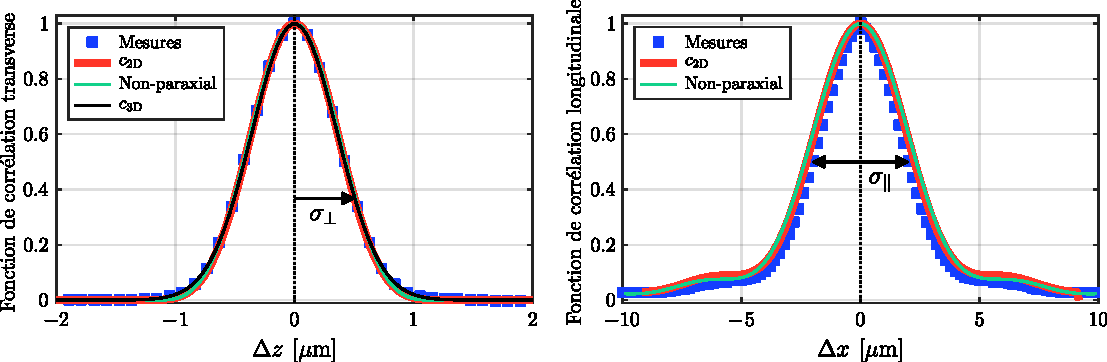
\includegraphics[width=\textwidth]{Fig/Speckle/speckle_correlations_exp.pdf}
\caption{\textbf{Corrélations spatiales du speckle.} Les données expérimentales (carrés bleus) sont comparés aux différents modèles. Le modèle non-paraxial (courbes vertes) développé par l'équipe de Dominique Delande permet de correctement décrire les corrélations expérimentales. Le modèle paraxial à ouverture numérique effective (courbes rouges) permet lui aussi de décrire correctement les corrélations mesurées, contrairement au modèle paraxial sans correction (courbes oranges). La fonction de corrélation transverse est similaire à une gaussienne (courbe noire), dont l'ajustement permet d'extraire la longueur de corrélation transverse $\sigmap=0.50\pm\SI{0.01}{\micro\metre}$ définie par le rayon à $1/e$. On définit la longueur de corrélation longitudinale $\sigmal=4.1\pm\SI{0.1}{\micro\metre}$ par la largeur totale à mi-hauteur des données expérimentales.}
\label{fig:speckle_correlations_exp}
\end{figure}





\paragraph*{Modèle à ouverture numérique effective}
Cependant, la mise en œuvre du modèle décrit par les équations \ref{eq:speckle_masque_phase} et \ref{eq:huygens_fresnel_num} est une procédure complexe autant numériquement qu'analytiquement, en particulier pour la détermination du spectre des fréquences spatiales du désordre $\widetilde{C}(\mathbf{k})$, déterminant pour décrire la dynamique du système. Ainsi, l'équipe a récemment développé un modèle plus simple, basé sur l'approximation paraxiale et faisant usage d'un facteur d'échelle géométrique $\xscale$ permettant de décrire une \emph{ouverture numérique effective} \citep{richard2019elastic}.

Dans le cadre de l'approximation paraxiale, on montre alors que la fonction de corrélation \ref{eq:correlation_3D_normalisee} aux alentours du plan de Fourier s'écrit
\begin{equation}
c_{\mathrm{3D}}(\Delta \mathbf{x}_\perp, \Delta z) \propto \left| \mathrm{TF} \left[ I_0'(\xzero) \: e^{i \pi \xzero^2 \Delta z /\lambda f^2} \right]_{\frac{\Delta \mathbf{x}_\perp}{\lambda f}} \right|^2 \text{ ,}
\label{eq:correlation_3D_paraxial_effectif}
\end{equation}
où le profil $I_0'(\xzero)$ d'intensité dans le plan du diffuseur vu sous l'ouverture numérique effective $\ON_{\mathrm{eff}}$ est donné par
\begin{equation}
I_0'(\xzero)= \exp{\left( -\frac{2 \xzero^2}{w_{\mathrm{eff}}^2} \right)} \: \Theta \left( \left| \xzero \right|- \frac{D_{\mathrm{eff}}}{2} \right)
\label{eq:profil_intensite_diffuseur}
\end{equation}
avec $\Theta(x)$ la fonction de Heaviside, et $D_{\mathrm{eff}}=\xscale D$ et $w_{\mathrm{eff}}=\xscale w$ les tailles caractéristiques effectives du faisceau. 

L'optimisation de la fonction de corrélation $c_{\mathrm{3D}}$ sur les données expérimentales permet de reproduire de manière fidèle les détails de notre désordre. De cette manière, on détermine que $\xscale=0.875\pm0.005$, donnant une ouverture numérique effective de $\ON_{\mathrm{eff}}=0.48\pm0.02$\footnote{Cette réduction de l'ouverture numérique provient des termes d'ordres supérieurs du développement limité de $\sin{\theta}$. Puisque $\left| \sin{\theta} \right|<\left|\theta\right|$, il convient d'utiliser un nouvel angle $\theta'<\theta$ de telle sorte que l'on retrouve la véritable valeur de l'ouverture numérique lorsque l'on utilise à nouveau l'approximation paraxiale $\sin{\theta'} \approx \theta'$}.



Le champ de speckle étant très étendu, la fonction de corrélation est très allongée selon la direction longitudinale comme décrit section \ref{sc:correlation_longitudinale}. La forme de la fonction de corrélation étant compliquée, la longueur de corrélation longitudinale est définie par la largeur totale à mi-hauteur\footnote{Le choix de cette définition a été fait par consistance avec le cas d'une illumination purement gaussienne, résultant en une fonction de corrélation longitudinale de forme lorentzienne.} $\sigmal=4.1\pm\SI{0.1}{\micro\metre}$. Cette définition entraîne alors un rapport d'aspect d'environ 8, témoignant de la forme très allongée des grains de speckle.




Pour terminer, précisons que les définitions des longueurs de corrélation utilisées dans ce manuscrit ne sont pas uniques. Notre présent choix est motivé pour des raisons de simplicité lors de l'étude du temps de diffusion élastique (voir chapitre \ref{ch:TauS_PRL}).%, cependant cette convention n'est pas celle la plus adaptée à l'étude des fonctions spectrales par exemple \citep{volchkov2018measurement}\citep{pasek2017anderson}. 














\section{Propriétés du potentiel de type speckle}
\label{sc:potentiel_speckle}
Jusqu'à ce point, nous nous sommes attachés à décrire le champ lumineux d'un \speckle . En particulier, nous avons montré le caractère granulaire de celui-ci, granularité dont la taille est donnée par la limite de diffraction. 

À présent, nous allons décrire comment l'intensité du champ de \speckle\ se traduit en terme de potentiel pour les atomes. 

\subsection{Propriétés du potentiel}
\label{sc:propriete_potentiel_speckle}
Comme annoncé en introduction de ce chapitre, le désordre nécessaire à l'étude de la propagation d'ondes de matière en milieux désordonnés est réalisé à l'aide du champ de \speckle\ décrit précédemment, dont l'effet sur les atomes est décrit par le potentiel dipolaire présenté section \ref{sc:forces_lumineuses}. En effet, l'effet d'un champ laser de pulsation $\omega$ et d'intensité $I(\mathbf{x})$ sur un atome à deux niveaux séparés par $\hb \omega_0$ est donné par \ref{eq:potentiel_dipolaire}, que l'on peut écrire plus simplement 
\begin{equation}
V(\mathbf{x}) \propto I(\mathbf{x}) \left( \frac{1}{\omega-\omega_0} - \frac{1}{\omega+\omega_0} \right) \text{ .}
\end{equation}
Comme décrit précédemment, le laser utilisé pour créer ce champ de \speckle\ est accordable autour de \SI{780}{\nano\metre}, c'est à dire proche de la résonance de la raie $D_2$ du \isotope[87]{Rb}. Dans ces conditions, il est possible d'appliquer l'approximation de l'onde tournante et de négliger le terme en $1/(\omega+\omega_0)$ devant le terme co-rotatif en $1/(\omega-\omega_0)$, le potentiel ressenti par les atomes s'exprimant alors
\begin{equation}
V(\mathbf{x}) \propto \frac{I(\mathbf{x})}{\delta} \text{ ,}
\label{eq:potentiel_dipolaire_approx}
\end{equation}
où $\delta=\omega-\omega_0$ est le désaccord du faisceau par rapport à la transition. 

Le potentiel désordonné ressenti par les atomes étant proportionnel à l'intensité lumineuse, il apparaît alors que les propriétés statistiques spatiales du potentiel sont exactement celles de l'intensité lumineuse du \speckle . Notamment, le potentiel généré par un \speckle\ est anisotrope et la taille typique des fluctuations de potentiel aux alentours du plan de Fourier est donnée par $\sigmap=\SI{0.5}{\micro\metre}$ dans le plan transverse et $\sigmal=\SI{4.1}{\micro\metre}$ dans la direction longitudinale, les fonctions de corrélations du potentiel et de l'intensité lumineuse étant identiques.

De plus, il a été montré dans la section précédente que le champ de \speckle\ n'est pas homogène, mais qu'il possède une extension finie. En particulier, l'équation \ref{eq:intensite_moyenne_speckle} stipule que le profil d'intensité moyenne est une gaussienne de waist $\speckleext\approx \SI{1.5}{\milli\metre}$, dont l'intensité au centre du faisceau dépend la puissance du laser $P$ selon
\begin{equation}
\overline{I}(\xf=0)=\frac{2P}{\pi \speckleext^2} \text{ ,}
\end{equation}
d'après les lois de l'optique gaussienne. Les tailles typiques des nuages utilisés étant au maximum de quelques dizaines de \SI{}{\micro\metre}, on peut supposer qu'à cette échelle, le potentiel moyen ressenti par les atomes est homogène et que sa valeur est fixée par l'intensité lumineuse au centre de la figure de \speckle : $\VR=\overline{V} \propto \overline{I}(\xf=0)/\delta$.

Une autre conséquence de l'expression \ref{eq:potentiel_dipolaire_approx} est qu'il est possible de créer un potentiel désordonné sur les atomes qui soit répulsif ($\delta>0$) ou bien attractif ($\delta<0$) selon le signe du désaccord $\delta$. Cette dernière possibilité nous permet d'avoir un degré de liberté expérimental supplémentaire, celui de la distribution de potentiel, dont l'importance sera illustrée dans les chapitres \ref{ch:TauS_PRL} et \ref{ch:TauS_NJP}. En effet, si la distribution de la norme du potentiel est fixée par celle de l'intensité lumineuse \ref{eq:proba_speckle}, ces deux quantités étant proportionnelles, le signe du désaccord nous permet de retourner la distribution de potentiel par rapport au potentiel nul $V=0$ (voir figure \ref{fig:distribution_potentiel})
\begin{equation}
\mathcal{P}(V)=\frac{1}{\left| \VR \right|} e^{-V/\VR} \cdot \Theta(V/\VR) \text{ ,}
\label{eq:distribution_potentiel_speckle}
\end{equation}
où $\Theta$ est la fonction de Heaviside valant 1 pour $V/\VR>0$, et 0 sinon. $\VR$ est le potentiel moyen, proportionnel à l'intensité lumineuse moyenne et dont le signe peut changer suivant celui du désaccord. L'amplitude du désordre est quant à elle donnée par l'écart-type de la distribution de potentiel $ \sigma_{V}=(\overline{V^2}-\overline{V}^2)^{1/2}=\left|\VR\right|>0$ et sera toujours positive. Ainsi, sur notre dispositif, changer l'amplitude du désordre revient simplement à faire varier la puissance du faisceau \speckle\ rayonné sur les atomes.


\begin{figure}
\centering
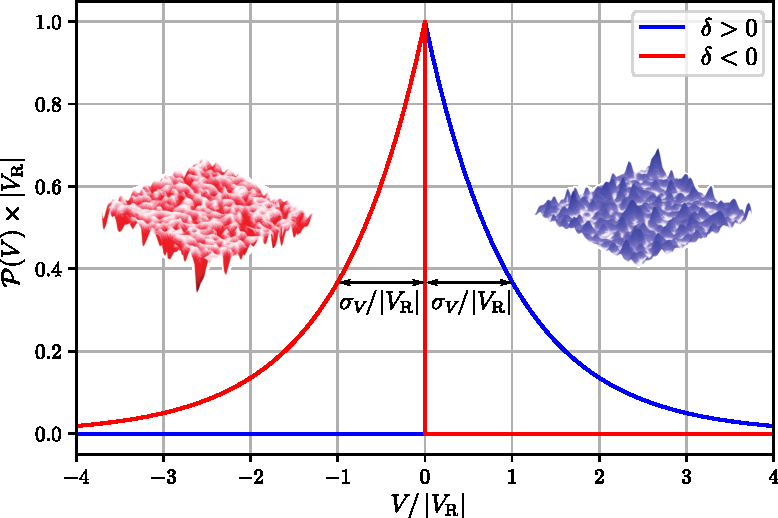
\includegraphics[width=0.85\textwidth]{Fig/Speckle/distribution_potentiel.pdf}
\caption{\textbf{Distributions de potentiel pour un désordre optique de type \speckle .} La distribution de potentiel suit celle de l'intensité lumineuse. Pour des désaccords positifs $\delta>0$, le potentiel créé est positif (illustration bleue) et sa distribution est une exponentielle décroissante (courbe bleue). Pour des désaccords négatifs $\delta<0$, le potentiel est alors attractif et ne peut dépasser 0 (illustration rouge). La distribution de potentiel est alors une exponentielle croissante (courbe en rouge).}
\label{fig:distribution_potentiel}
\end{figure}






\subsection{Possibilité d'un potentiel dépendant de l'état interne}
\label{sc:state_dependent_disorder}
Comme nous l'avons au cours du chapitre \ref{ch:Localisation}, l'étude du régime critique de la transition d'Anderson nécessite de pouvoir adresser sélectivement les différents niveaux d'énergie du désordre. Il s'agit donc de procéder à une spectroscopie du désordre. Pour cela, nous devons disposer d'un état libre dans lequel nous préparons notre condensat de Bose-Einstein, c'est à dire insensible au potentiel désordonné, et d'un second état couplé au désordre. Dans cette section, on s'attachera donc à décrire la notion de potentiel dépendant de l'état interne des atomes.

\paragraph*{Principe du désordre dépendant de l'état interne}
Comme explicité section \ref{sc:forces_lumineuses}, la formule \ref{eq:potentiel_dipolaire} décrivant le potentiel dipolaire a été obtenue dans la limite des grands désaccords pour un système à deux niveaux, ne tenant donc compte ni de la structure fine, ni de la structure hyperfine du \isotope[87]{Rb}. En particulier, la structure hyperfine de l'état fondamental $5^2S_{1/2}$ possède deux niveaux $\etatF{1}{}$ et $\etatF{2}{}$ séparés de $\deltahf=\SI{6.83}{\giga\hertz}$ très grande devant la largeur de la transition $\Gamma/2\pi=\SI{6.07}{\mega\hertz}$. 

En fixant le désaccord $\delta_{\mathrm{2,F'}}$ par rapport à la transition $\etatF{2}{}\rightarrow \etat{F'}$ de telle sorte que celui-ci soit très petit devant la séparation hyperfine des états fondamentaux $\left| \delta_{\mathrm{2,F'}} \right| /2 \pi \ll \deltahf$, on peut réaliser un potentiel dont la valeur moyenne dépend de l'état interne:
\begin{equation}
\overline{V_2} \propto \frac{\overline{I}}{\delta_{\mathrm{2,F'}}/2\pi} \quad \text{et} \quad \overline{V_1} \propto \frac{\overline{I}}{\delta_{\mathrm{2,F'}}/2\pi+\deltahf} \text{ .}
\end{equation}
Avec la condition d'un petit désaccord, on obtient alors $\left| \overline{V_1} \right| \ll \left| \overline{V_2} \right|$, comme illustré figure \ref{fig:principe_potentiel_etat_interne}. On dispose donc d'un moyen de réaliser un potentiel conséquent sur l'état $\etatF{2}{}$ tout en rendant celui ressenti par l'état $\etatF{1}{}$ négligeable, état dans lequel nous préparons notre condensat de Bose-Einstein.


\begin{figure}
\centering
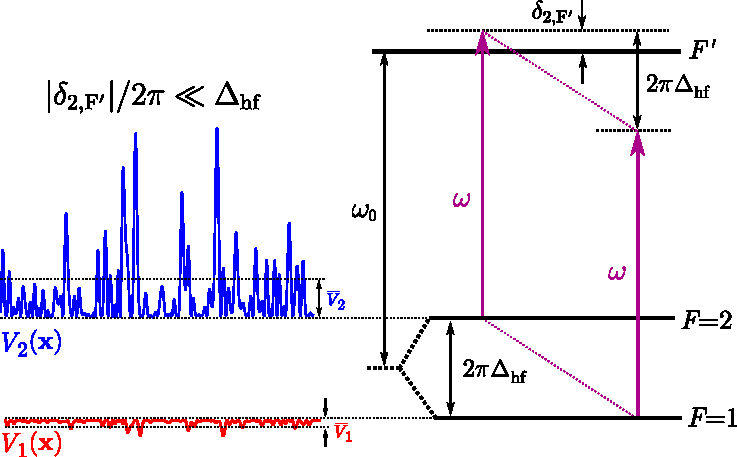
\includegraphics[width=0.8\textwidth]{Fig/Speckle/principe_potentiel_etat_interne.pdf}
\caption{\textbf{Réalisation d'un potentiel dépendant de l'état interne.} Le choix d'un désaccord $\delta_{\mathrm{2,F'}}$ par rapport à la transition $\protect\etatF{2}{} \rightarrow \protect\etat{F'}$ qui soit petit devant la séparation hyperfine $2\pi\deltahf$ des états $\protect\etatF{1}{}$  et $\protect\etatF{2}{}$ permet de soumettre un potentiel aux atomes dans l'état $\protect\etatF{2}{}$ tout en rendant celui ressenti par les atomes dans l'état $\protect\etatF{1}{}$ négligeable. Le choix du signe du désaccord $\delta_{\mathrm{2,F'}}$ permet de plus de contrôler le caractère attractif ($\delta_{\mathrm{2,F'}}<0$) ou répulsif ($\delta_{\mathrm{2,F'}}>0$) du potentiel.}
\label{fig:principe_potentiel_etat_interne}
\end{figure}


\paragraph*{Détails du potentiel dipolaire}
À l'échelle des désaccords typiques recherchés dans une telle situation (de l'ordre de \SI{100}{\mega\hertz}), il est aussi nécessaire de tenir compte de la structure hyperfine de l'état excité $5^2 P_{3/2}$ du \isotope[87]{Rb}, qui se décompose en quatre états hyperfins $\etat{F'=\lbrace 0,1,2,3 \rbrace}$. On peut alors montrer que le potentiel dipolaire ressenti par les états fondamentaux $\etatF{1}{}$ et $\etatF{2}{}$ est la somme des contributions de chacune des transitions vers un état excité \citep{grimm2000optical}. 

De plus, le faisceau \speckle\ étant polarisé linéairement suivant l'axe du champ magnétique $\vec{y}$, les contributions au potentiel dipolaire se restreignent aux transitions $\pi$ ($\Delta\mf=0$) et on peut alors montrer à l'aide d'un calcul attentif de la polarisabilité atomique que le potentiel dipolaire ressenti par les états fondamentaux hyperfins est donné par \citep{denechaud2018vers, grimm2000optical, steck2001rubidium}:
\begin{equation}
V_2(\mathbf{x}) = \frac{3 \pi c^2 \Gamma I(\mathbf{x})}{\omega_0^3} \left( \frac{1}{40 \: \delta_{2,1}} + \frac{1}{24 \: \delta_{2,2}} + \frac{4}{15 \: \delta_{2,3}} \right) 
\label{eq:potentiel_dipolaire_hyperfin_V2}
\end{equation}
et
\begin{equation}
V_1(\mathbf{x}) = \frac{3 \pi c^2 \Gamma I(\mathbf{x})}{\omega_0^3} \left( \frac{5}{24 \: \delta_{1,1}} + \frac{1}{8 \: \delta_{1,2}} \right) \text{ ,}
\label{eq:potentiel_dipolaire_hyperfin_V1}
\end{equation}
où les quantités $\delta_{\mathrm{F,F'}}$ correspondent aux désaccords en \SI{}{\radian\per\second} associés à chacune des transitions $\etat{F,\mf} \rightarrow \etat{F',\mf'=\mf}$. En prenant la transition $\etat{F=2} \rightarrow \etat{F'=3}$ comme référence, on peut tracer l'évolution du potentiel dipolaire pour l'état $\etat{F=2}$ en fonction du désaccord $\delta_{2,3}$, les autres désaccords étant déductibles de la structure hyperfine des états excités. Cette évolution est représentée figure \ref{fig:potentiel_dipolaire_hyperfin}, qui comporte trois divergences du potentiel correspondant aux trois transitions $\pi$ possibles $\etat{F=2} \rightarrow \etat{F'=\lbrace 1,2,3 \rbrace}$.


\begin{figure}
\centering
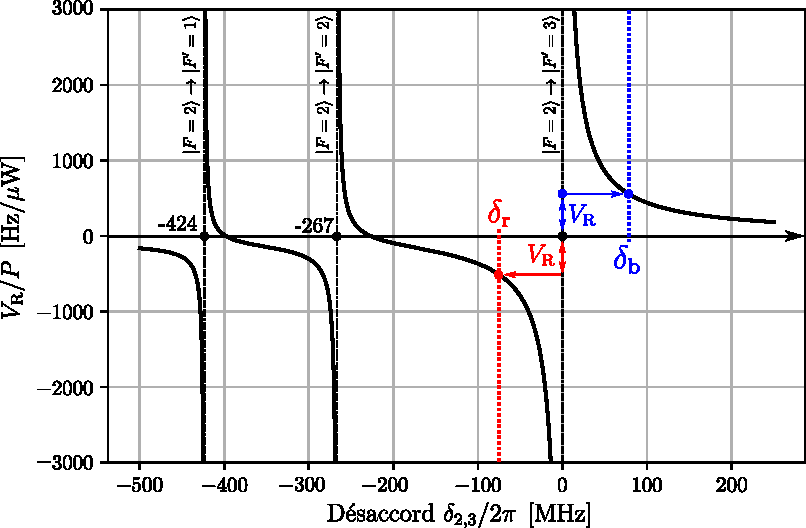
\includegraphics[width=0.9\textwidth]{Fig/Speckle/potentiel_dipolaire_hyperfin.pdf}
\caption{\textbf{Potentiel dipolaire $\overline{V_2}$ dû à la structure hyperfine du \isotope[87]{Rb}.} En fixant la puissance du faisceau \speckle\ dont l'extension est donnée par $\speckleext$, le potentiel moyen $\VR=\overline{V_2}$ ressenti par l'état $\protect\etatF{2}{}$ évolue avec le désaccord $\delta_{2,3}$ par rapport à la transition $\protect\etatF{2}{} \rightarrow \etat{F'=3}$. Les trois divergences de potentiel observées correspondent aux trois transitions $\pi$ possibles.}
\label{fig:potentiel_dipolaire_hyperfin}
\end{figure}

À l'instar du cas d'un potentiel réalisé à l'aide d'un désaccord suffisamment grand devant la structure hyperfine du \isotope[87]{Rb} présenté dans la section \ref{sc:propriete_potentiel_speckle} précédente, la figure \ref{fig:potentiel_dipolaire_hyperfin} illustre la possibilité de réaliser des potentiels qui soient attractifs ou répulsifs en sélectionnant soigneusement le désaccord du laser par rapport à la transition $\etat{F=2} \rightarrow \etat{F'=3}$\footnote{La sélection de cette transition comme référence s'explique par sa forte contribution au potentiel ressenti par l'état $\protect\etatF{2}{}$ comme explicité équation \ref{eq:potentiel_dipolaire_hyperfin_V2}. Ceci est aussi visible sur la figure \ref{fig:potentiel_dipolaire_hyperfin} où l'effet de cette transition apparaît sur une bande d'environ $\pm\SI{200}{\mega\hertz}$, bien plus large que pour les deux autres transitions.}. Dans cet exemple, les désaccords $\delta_{2,3}=\delta_{\mathrm{r}}=-2\pi \times \SI{73}{\mega\hertz}$  et $\delta_{2,3}=\delta_{\mathrm{b}}=2\pi \times \SI{81}{\mega\hertz}$ choisis permettent tous deux d'obtenir un potentiel moyen $\left|\VR\right| /P=h\times\SI{0.32}{\kilo\hertz/\micro\watt}$\footnote{Il ne s'agit ici que d'une estimation photométrique. Si le choix des désaccords $\delta_{\mathrm{r}}$ et $\delta_{\mathrm{b}}$ est réalisé expérimentalement en mesurant les déplacements lumineux dus au faisceau homogène, la puissance du faisceau \speckle\ au niveau des atomes est estimée à l'aide de la transmission de chaque élément optique et de la troncature du faisceau par la monture du diffuseur. Cette "calibration" n'est donc qu'une estimation.} où $\VR=\overline{V_2}$ est le potentiel moyen ressenti par l'état $\etat{F=2}$. À l'aide des équations \ref{eq:potentiel_dipolaire_hyperfin_V2} et \ref{eq:potentiel_dipolaire_hyperfin_V1}, on détermine alors que le choix de tels désaccords pour des désordres attractifs ($\delta_{\mathrm{r}}<0$) ou bien répulsifs ($\delta_{\mathrm{b}}>0$) donne un rapport de potentiels de l'ordre de 
\begin{equation}
\left|V_1 \right| / \left| V_2 \right| \approx 1/66 \text{ ,}
\label{eq:ratio_desordre_etat}
\end{equation}
montrant donc la très forte différence entre les potentiels ressentis par les deux états fondamentaux de notre espèce atomique. La mise en œuvre expérimentale d'un tel désordre dépendant de l'état interne des atomes a permis la mesure des fonctions spectrales \citep{volchkov2018measurement}, dont les grandes lignes seront décrites dans le chapitre \ref{ch:TauS_NJP}. %Une discussion complète des détails de mesures peut être retrouvée dans la thèse de Vincent Denechaud \citep{denechaud2018vers}.

\paragraph*{Implémentation expérimentale}
L'utilisation d'un tel potentiel proche de résonance impose certaines contraintes quant à la puissance et à la fréquence du laser utilisé. En particulier, il est nécessaire de stabiliser la fréquence du laser afin de réduire au maximum les fluctuations du potentiel étant donné le faible désaccord ($\left|\delta_{2,3}\right|/2\pi\sim\SI{80}{\mega\hertz}$).

Une spécificité de notre montage réside dans sa capacité à stabiliser des très faibles puissances optiques\footnote{L'exemple du paragraphe précédent montre que des fluctuations de puissance de l'ordre de \SI{1}{\micro\watt} peut engendrer des fluctuations de potentiel de \SI{500}{\hertz}.}. Pour cela, le montage de mise en forme du faisceau est très similaire à celui présenté section \ref{sc:montage_diffuseur} où l'accent a été mis sur la contrainte de l'utilisation de très faibles puissances optiques, voir figure \ref{fig:montage_speckle_specfunc}. La lame séparatrice utilisée pour la stabilisation de puissance permet de dévier 90\% de la puissance vers la photodiode, permettant ainsi d'obtenir une grande sensibilité aux fluctuations de puissance. Les 10\% transmis sont ensuite atténués à l'aide d'une densité optique \emph{Thorlabs NE30A-B} permettant de diviser la puissance d'un facteur 1000. Les puissances alors obtenues sont stabilisées et contrôlables entre typiquement \SI{30}{\nano\watt} et \SI{15}{\micro\watt}.

\begin{figure}
\centering
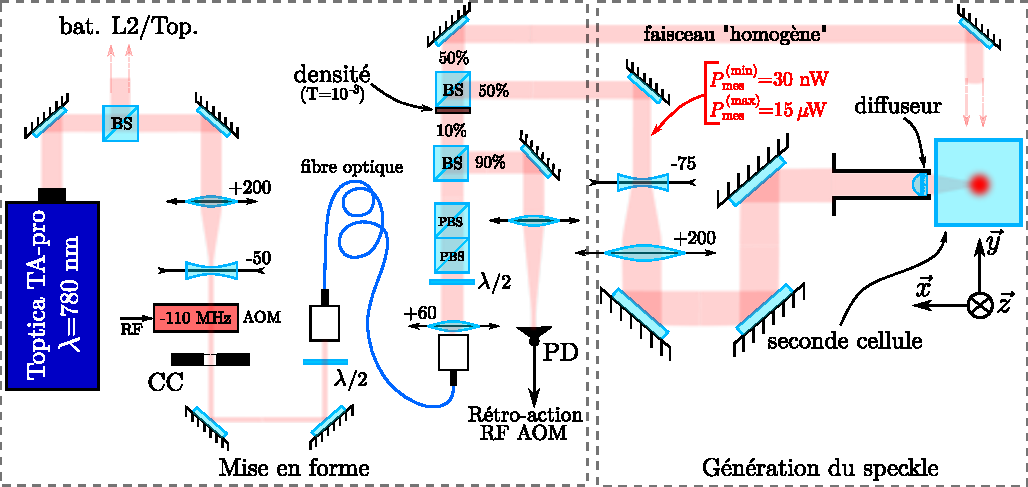
\includegraphics[width=\textwidth]{Fig/Speckle/montage_speckle_specfunc.pdf}
\caption{\textbf{Montage \speckle\ pour un désordre dépendant de l'état interne.} L'approche de désordre dépendant de l'état interne nécessitant de très faibles puissances optiques, le montage précédent a été adapté afin de pouvoir stabiliser des puissances de l'ordre du \SI{}{\micro\watt} à l'aide d'une densité optique atténuant fortement le faisceau. L'utilisation de 90\% de la puissance du faisceau pour la stabilisation en puissance permet d'obtenir une meilleure sensibilité aux fluctuations de puissance. De plus, la fréquence du faisceau laser est stabilisée par battements avec le laser repompeur \emph{L2}.}
\label{fig:montage_speckle_specfunc}
\end{figure}


\paragraph*{Limitation du potentiel résiduel sur l'état $\etatF{1}{}$}
Une conséquence de l'équation \ref{eq:ratio_desordre_etat} est la suivante. Bien que le potentiel moyen $\overline{V_1}$ ressenti par l'état $\etatF{1}{}$ soit faible, celui-ci ne s'annule pas exactement. Quelle limite peut-on alors donner à la force du désordre $\VR$? Pour cela intéressons-nous à la limite que l'on peut donner au potentiel résiduel $V_1$. 


Nous avons vu section \ref{sc:propriete_BEC} que pour un condensat de Bose-Einstein dans le régime de Thomas-Fermi, les interactions entre particules écrantent le potentiel externe soumis aux atomes. Il en résulte que sur l'ensemble du condensat, l'énergie des atomes est constante et égale au potentiel chimique $\mu$. Ainsi, pour un potentiel désordonné résiduel d'amplitude faible $\overline{V_1}\ll\mu$, une petite modulation de densité du condensat permet de compenser l'effet de ce potentiel. Ainsi, l'énergie potentielle de chaque atome reste constante et égale au potentiel chimique. Dans ces conditions, le potentiel résiduel $\overline{V_1}$ ne perturbe pas l'état libre $\etatF{1}{}$.



Augmentons alors la force du désordre: le potentiel résiduel augmente jusqu'à ce que celui-ci dépasse par endroits le potentiel chimique. À ces endroits, l'énergie d'interaction n'est plus suffisante pour écranter l'énergie potentielle du désordre et on crée un trou dans le condensat. Notons de plus que localement l'énergie ne sera plus égale au potentiel chimique. La conséquence la plus néfaste est l'apparition de nouvelles énergies dans la distribution d'énergie de l'état libre, dégradant ainsi la spectroscopie recherchée.

Le caractère limitant du désordre résiduel apparaît donc lorsque celui-ci est de l'ordre du potentiel chimique $\overline{V_1} \lesssim \mu \approx h\times\SI{40}{\hertz}$\footnote{La détermination exacte de la limite applicable fait aussi intervenir la longueur de cicatrisation du condensat ainsi que la longueur de corrélation du potentiel. Le raisonnement présenté ici permet de tout même d'expliquer qualitativement l'origine de cette limitation.}. En utilisant le rapport \ref{eq:ratio_desordre_etat}, on estime alors que le désordre maximal applicable à l'aide de cette technique est de l'ordre de quelques $h\times\SI{}{\kilo\hertz}$\footnote{Cet effet a été observé lors de la mesure des fonctions spectrales \citep{denechaud2018vers, volchkov2018measurement}.}. 











\section{Potentiel composé d'un \speckle\ bichromatique}
\label{sc:speckle_bichromatique}
Comme nous avons pu le voir dans la section \ref{sc:spectroscopie_transition}, le protocole expérimental envisagé pour l'étude la transition d'Anderson comporte deux étapes: une première étape de chargement d'états du désordre à énergie résolue est suivie de la caractérisation de ces états en terme de localisation. 

Si l'approche décrite dans la section précédente permet de réaliser une spectroscopie du potentiel désordonné appliqué aux atomes, celle-ci ne permet pas d'étudier la transition d'Anderson dans la mesure où celle-ci nécessite de réaliser des expériences d'expansion du nuage suite à la spectroscopie. 

La principale limitation de cette approche provient du faible désaccord du faisceau \speckle . En effet, les désaccords utilisés étant de l'ordre de $\left|\delta \right| \approx 12 \Gamma$, le taux d'émission spontanée est relativement grand. Cela conduit à un temps de vie maximal des atomes habillés par le désordre d'une centaine de millisecondes, très insuffisant pour les temps d'expansions visés de plus d'une seconde.

Il est donc nécessaire de trouver une nouvelle façon de créer un désordre dépendant de l'état interne avec une durée de vie suffisante pour pouvoir procéder à des expériences d'expansion. 


\subsection{S'éloigner de résonance}
\label{sc:speckle_bichromatique_mukhtar}
L'approche intuitive pour diminuer le taux d'émission spontanée consiste à s'éloigner de la transition atomique, et donc à augmenter le désaccord. En effet, il est possible d'obtenir une estimation du taux d'émission spontanée $\Gamma_2$ de l'état $\etatF{2}{}$ à l'aide de
\begin{equation}
\Gamma_2 \approx \frac{1}{\hb} \left[ \VR \right| \frac{\Gamma}{\left|\delta\right|} \text{ ,}
\end{equation}
où $\Gamma=2\pi \times \SI{6.07}{\mega\hertz}$ correspond à la largeur de la transition $D_2$ du \isotope[87]{Rb} et $\delta$ est le désaccord.

Afin d'obtenir un temps de vie $\Gamma_2^{-1}$ de l'ordre de la seconde pour un désordre d'environ \SI{500}{\hertz} typiquement utilisé sur l'expérience, il est nécessaire d'utiliser un désaccord de plusieurs \SI{}{\giga\hertz}. Cette condition est donc incompatible avec celle de désordre dépendant de l'état interne dans la mesure où les potentiels $\overline{V_1}\sim\overline{V_2}$ deviennent comparables pour de tels désaccords.


La question est alors la suivante: est-il possible de réaliser un désordre dépendant de l'état interne tout en ayant un taux d'émission spontanée suffisamment faible pour permettre l'étude de la localisation d'Anderson?


\paragraph*{Speckle bichromatique}
La réponse apportée par l'équipe pour augmenter le temps de vie des atomes vis-à-vis de l'émission spontanée consiste à utiliser des désaccords plus importants, de l'ordre de \SI{100}{\giga\hertz}. %Cependant, l'utilisation de désaccords aussi grands ($\delta/2\pi \gg \deltahf$) ne permet plus la sélectivité en état interne recherchée pour réaliser une spectroscopie du désordre. 
L'idée est alors de compenser le potentiel ressenti par l'état $\etatF{1}{}$ à l'aide d'une seconde fréquence optique, comme l'illustre la figure \ref{fig:speckle_bichromatique_repulsif}. Une étude quantitative et détaillée de cette approche peut être retrouvée dans le manuscrit de thèse de Musawwadah Mukhtar \citep{mukhtar2019state}, aussi nous nous contenterons de décrire les grandes lignes de cette approche. 

\begin{figure}
\centering
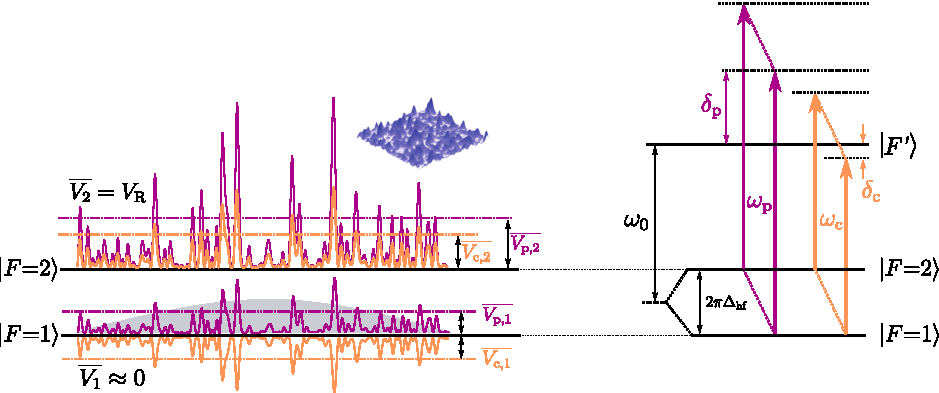
\includegraphics[width=\textwidth]{Fig/Speckle/speckle_bichromatique_repulsif.pdf}
\caption{\textbf{Illustration du principe de \speckle\ bichromatique dans le cas d'un désordre répulsif.} Un laser principal de désaccord $\delta_{\mathrm{p}}$ important soumet les deux états fondamentaux à un potentiel similaire (lignes bordeaux). Afin d'obtenir un potentiel dépendant de l'état interne, on utilise une seconde fréquence optique générée par un laser de compensation de désaccord $\delta_{\mathrm{c}}$ (lignes oranges) dans le but de compenser le potentiel créé par le laser principal sur l'état $\protect\etatF{1}{}$ dans lequel est créé le condensat (zone grisée). Dans le cas d'un désordre répulsif comme illustré ici (voir miniature bleue), il est de plus possible d'additionner les effets répulsifs des potentiels créés par ces deux lasers sur l'état $\protect\etatF{2}{}$.}
\label{fig:speckle_bichromatique_repulsif}
\end{figure}




Le désordre soumis aux atomes résulte alors de la superposition de deux figures de \speckle , générées par deux lasers. Un laser \emph{principal} grandement désaccordé crée un potentiel comparable sur les états $\etatF{1}{}$ et $\etatF{2}{}$. Un laser de \emph{compensation} crée un second potentiel de telle sorte que son effet sur l'état $\etatF{1}{}$ soit de compenser le potentiel du laser principal (voir figure \ref{fig:speckle_bichromatique_repulsif}). 

Dans le cadre de la théorie de la réponse linéaire, on montre à l'aide de la partie réelle de la polarisabilité atomique que le potentiel moyen total ressenti par chaque état est la somme des potentiels générés par chaque laser. Ces potentiels sont alors donnés par:
\begin{equation}
\overline{V_1}=\overline{V_{\mathrm{p},1}}+\overline{V_{\mathrm{c},1}}=0 \quad \text{et} \quad
\overline{V_2}=\overline{V_{\mathrm{p},2}}+\overline{V_{\mathrm{c},2}}=\VR \text{ ,}
\label{eq:contraintes_potentiel_bichromatique}
\end{equation}
avec $\overline{V_{\mathrm{p},i}}$ ($\overline{V_{\mathrm{c},i}}$) le potentiel moyen créé par le laser principal (de compensation) sur l'état $\etatF{i}{}$. Nous avons de plus fait apparaître la contrainte que le potentiel moyen total appliqué à l'état $\etatF{1}{}$ soit nul. De même, les taux d'émission spontanée s'additionnent, ceux-ci étant issus de la partie imaginaire de la polarisabilité atomique: 
\begin{equation}
\Gamma_{\mathrm{sp},1}=\Gamma_{\mathrm{sp,p},1} + \Gamma_{\mathrm{sp,c},1} \quad \text{et} \quad \Gamma_{\mathrm{sp},2}=\Gamma_{\mathrm{sp,p},2} + \Gamma_{\mathrm{sp,c},2} \text{ ,}
\label{eq:temps_vie_desordre}
\end{equation}
avec $\Gamma_{\mathrm{sp},i}$ le taux d'émission spontanée pour l'état $\etatF{i}{}$.

Afin de pouvoir étudier la dynamique des atomes dans le désordre pendant de très longs temps d'expansions, il est nécessaire de maximiser le temps de vie de l'état $\etatF{2}{}$. Cependant, cette procédure tend à diminuer le temps de vie de l'état $\etat{F=1}$, qui doit être suffisamment long pour pouvoir réaliser l'étape de \emph{chargement} du désordre. Le but de cette étude est alors d'optimiser les temps de vie \ref{eq:temps_vie_desordre} des deux états pour un désordre $\VR$ fixé, tout en respectant les contraintes \ref{eq:contraintes_potentiel_bichromatique} du potentiel. Expérimentalement, nous disposons de quatre degrés de liberté (la puissance et le désaccord de chaque \speckle) pour atteindre la configuration optimale. %En particulier, les désaccords des deux faisceaux doivent satisfaire des conditions afin de permettre l'approche de désordre dépendant de l'état interne.

\paragraph*{Potentiel répulsif}
Considérons tout d'abord le cas d'un désordre répulsif sur l'état $\etatF{2}{}$, qui correspond à celui illustré sur la figure \ref{fig:speckle_bichromatique_repulsif}. Le laser principal étant grandement désaccordé, le potentiel moyen que celui-ci induit sur les états $\etatF{1}{}$ et $\etatF{2}{}$ est similaire. En prenant comme référence la transition $\etatF{1}{}\rightarrow\etat{F'}$\footnote{En choisissant un désaccord de \SI{100}{\giga\hertz}, on peut négliger la structure hyperfine de l'état excité.}, le désaccord du laser principal satisfait alors la condition $\delta_{\mathrm{p}}>0$\footnote{En prenant comme référence la transition $\protect\etatF{2}{}\rightarrow\protect\etat{F'}$, cette condition devient $\delta_{\mathrm{p}}/2\pi>\deltahf$.}, pour laquelle le potentiel généré sur les deux états hyperfins est répulsif. 

Afin de compenser le potentiel répulsif induit par le laser principal sur l'état $\etatF{1}{}$, il est nécessaire que le laser de compensation réalise un potentiel attractif, impliquant alors que le désaccord soit négatif $\delta_{\mathrm{c}}<0$\footnote{Pour les désaccords supérieurs au \SI{}{\giga\hertz} considérés, nous pourrons négliger le détail de la structure hyperfine de l'état excité, large de \SI{229}{\mega\hertz} pour les états accessibles.}. Notons de plus que le choix d'un désaccord inférieur à la séparation hyperfine des états fondamentaux permet de générer un potentiel répulsif sur l'état $\etatF{2}{}$. On retiendra alors:
\begin{equation}
\delta_{\mathrm{p}}>0 \quad \text{et} \quad -\deltahf<\delta_{\mathrm{c}}/2\pi<0 
\label{eq:condition_desordre_repulsif}
\end{equation}
comme configuration pour un désordre bichromatique répulsif.

\paragraph*{Potentiel attractif}
Considérons à présent le cas d'un potentiel attractif pour l'état $\etatF{2}{}$. De même que dans le cas répulsif, le laser principal est très désaccordé, cependant son désaccord doit être négatif pour les deux états fondamentaux $\delta_{\mathrm{p}}/2\pi<-\deltahf$ en prenant la transition $\etatF{1}{}\rightarrow\etat{F'}$ comme référence. 

La principale différence provient ici du laser de compensation, qui ne peut pas générer à la fois un potentiel attractif pour l'état $\etatF{2}{}$ et un potentiel répulsif qui pourrait compenser le potentiel attractif du laser principal sur l'état $\etatF{1}{}$. La contrainte d'annulation du potentiel sur l'état initial impose alors le choix d'un désaccord positif $\delta_{\mathrm{c}}>0$ du laser de compensation par rapport à la transition $\etatF{1}{}\rightarrow\etat{F'}$. Le choix d'un potentiel total attractif sur l'état $\etatF{2}{}$ impose donc:
\begin{equation}
\delta_{\mathrm{p}}/2\pi<-\deltahf \quad \text{et} \quad \delta_{\mathrm{c}}>0 \text{ .}
\label{eq:condition_desordre_attractif}
\end{equation}

\begin{figure}
\centering
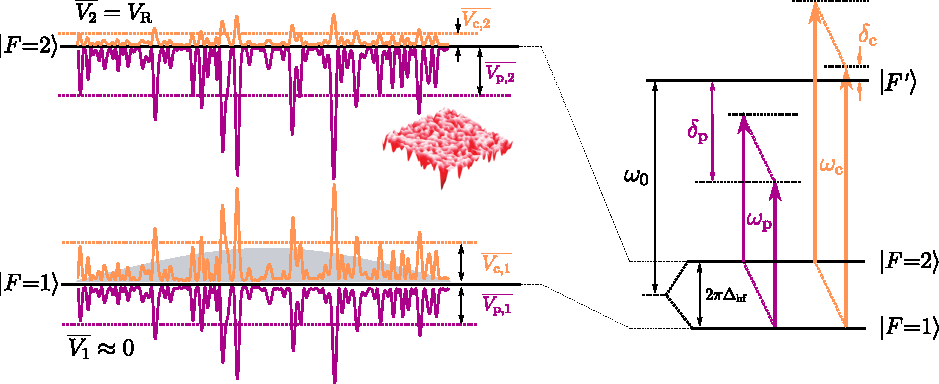
\includegraphics[width=\textwidth]{Fig/Speckle/speckle_bichromatique_attractif.pdf}
\caption{\textbf{Configuration du \speckle\ bichromatique dans le cas d'un désordre attractif.} Un laser principal de désaccord $\delta_{\mathrm{p}}$ important soumet les deux états fondamentaux à un potentiel similaire attractif (lignes bordeaux). Afin d'obtenir un potentiel dépendant de l'état interne, on utilise une seconde fréquence optique générée par un laser de compensation de désaccord $\delta_{\mathrm{c}}>0$ (lignes oranges) dans le but de compenser le potentiel créé par le laser principal sur l'état $\protect\etatF{1}{}$. Dans le cas d'un désordre attractif comme illustré ici (voir miniature rouge), la sélectivité de l'état interne ne se fait que par déséquilibre des potentiels sur l'état $\protect\etatF{2}{}$.}
\label{fig:speckle_bichromatique_attractif}
\end{figure}

Contrairement au cas répulsif, la sélectivité en état interne dans le cas attractif provient donc d'un déséquilibrage des potentiels sur l'état $\etatF{2}{}$, voir figure \ref{fig:speckle_bichromatique_attractif}.


\paragraph*{Performances d'un désordre bichromatique}
Si l'optimisation de la durée de vie $\Gamma_2^{-1}$ est d'importance capitale pour procéder aux mesures d'expansion des atomes chargés dans le désordre, il est tout de même nécessaire que les atomes dans l'état $\etatF{1}{}$ possèdent un temps de vie $\Gamma_1^{-1}$ suffisamment grand devant la durée du transfert spectroscopique. Nous verrons section \ref{sc:mesure_fonction_spectrale} que pour les désordres utilisés les plus forts, les temps de couplage radio-fréquence entre les états $\etatF{1}{}$ et $\etatF{2}{}$ sont de l'ordre de \SI{10}{\milli\second}. Ceci impose donc:
\begin{equation}
\Gamma_1^{-1}\geq\SI{10}{\milli\second} \text{ .}
\end{equation}

Aussi, nous choisissons de fixer le désaccord du laser principal à $\delta_{\mathrm{p}}= \pm 2\pi\times\SI{100}{\giga\hertz}$. Ce choix permet de réduire la complexité de la détermination des trois autres degrés de liberté expérimentaux $\delta_{\mathrm{c}}$, $P_{\mathrm{p}}$ et $P_{\mathrm{c}}$.

La table \ref{tb:speckle_bichromatique} présente les résultats de la détermination des paramètres optimisant le temps de vie $\Gamma_2^{-1}$ de l'état $\etatF{2}{}$. Cette étude a été menée pour un désordre d'amplitude $\VR/h=\SI{4}{\kilo\hertz}$, correspondant au désordre le plus extrême utilisé lors de la mesure des fonctions spectrales. L'optimisation des paramètres expérimentaux permet alors d'obtenir un temps de vie $\Gamma_2^{-1}$ de l'ordre de \SI{150}{\milli\second}. Comparé au temps de vie de \SI{0.4}{\milli\second} obtenu avec un speckle monochromatique, ceci représente une amélioration de près de trois ordres de grandeur. 



\begin{table}[!h]
\begin{center}
{\rowcolors{2}{white}{MainColor!10}
\begin{tabular}{ c|c|c }
%\hline
 & {\color{MainColor}\textbf{Désordre attractif}} & {\color{MainColor}\textbf{Désordre répulsif}} \\ [2ex]
%\hline
\textbf{Paramètres fixés} & & \\
Amplitude du désordre $\VR$ & $-h\times \SI{4}{\kilo\hertz}$ & $h\times\SI{4}{\kilo\hertz}$ \\
Désaccord du laser principal $\delta_{\mathrm{p}}$ & $-2\pi\times \SI{100}{\giga\hertz}$ & $2\pi\times\SI{100}{\giga\hertz}$ \\
Temps de vie $\Gamma_1^{-1}$ & \SI{10}{\milli\second} & \SI{10}{\milli\second} \\ [2ex]
%\hline
\textbf{Paramètres déterminés} & & \\
Désaccord du laser de compensation $\delta_{\mathrm{c}}$ & $2\pi \times \SI{1.354}{\giga\hertz}$ & $-2\pi \times \SI{1.622}{\giga\hertz}$ \\
%\hline
Puissance du laser principal $P_{\mathrm{p}}$ & \SI{8.14}{\milli\watt} & \SI{5.16}{\milli\watt} \\
%\hline
Puissance du laser de compensation $P_{\mathrm{c}}$ & \SI{130.2}{\micro\watt} & \SI{69.6}{\micro\watt} \\
%\hline
Temps de vie $\Gamma_2^{-1}$ & \SI{165}{\milli\second} & \SI{149}{\milli\second} \\
%\hline
\end{tabular}}
\end{center}
\caption{\textbf{Paramètres expérimentaux optimisés pour un désordre de 4~kHz.} La détermination de ces paramètres est détaillée dans la thèse Musawwadah Mukhtar \citep{mukhtar2019state}. Cette étude est menée pour le désordre le plus extrême utilisé pour la mesure des fonctions spectrales \citep{volchkov2018measurement} pour lequel le temps de vie $\Gamma_2^{-1}$ n'était que \SI{0.4}{\milli\second}. On remarque que les conditions \ref{eq:condition_desordre_repulsif} et \ref{eq:condition_desordre_attractif} sont vérifiées.}
\label{tb:speckle_bichromatique}
\end{table}





\paragraph*{Augmenter encore plus le temps de vie}
Si les potentiels générés par les deux faisceaux sur l'état $\etatF{1}{}$ sont d'amplitudes semblables (l'annulation du potentiel total sur $\etatF{1}{}$ ne serait pas possible autrement), on comprend aisément que le laser de compensation contribue fortement à la dissipation par émission spontanée compte-tenu de son petit désaccord en comparaison de celui du laser principal.

Cependant, après l'étape de chargement, une fois les atomes transférés dans l'état $\etatF{2}{}$ habillé par le désordre, il n'est plus nécessaire de compenser le potentiel vu par l'état $\etatF{1}{}$. Il est alors possible de s'affranchir du laser de compensation. Un moyen simple d'augmenter le temps de vie $\Gamma_2^{-1}$ consiste alors à diminuer progressivement la puissance du laser de compensation tout en modifiant celle du laser principal de manière à garder $\VR$ constant, comme illustré figure \ref{fig:sequence_spectro_transition}. Dans le cas d'un désordre répulsif, cela se traduit par l'augmentation de la puissance du laser principal $P_{\mathrm{p}}'$ tel que:
\begin{equation}
P_{\mathrm{p}}'=P_{\mathrm{p}}\times\VR/\overline{V_{\mathrm{p,2}}} \text{ .}
\end{equation}
%Il s'agit, après chargement dans le désordre, d'un moyen de s'éloigner encore plus de résonance.

On montre alors que le nouveau temps de vie $\Gamma_2^{'-1}$ de l'état $\etatF{2}{}$ après extinction du laser de compensation est donné par \citep{mukhtar2019state}:
\begin{equation}
\Gamma_2^{'-1}=\Gamma_2^{-1} \frac{\overline{V_{\mathrm{p},2}}/\VR}{\Gamma_{\mathrm{p},2}/\Gamma_2} \text{ .}
\end{equation}
L'application à un désordre d'amplitude $\left|\VR\right|/h=\SI{4}{\kilo\hertz}$ fournit alors un temps de vie de \SI{0.68}{\second} pour un désordre attractif et de \SI{0.69}{\second} pour un désordre répulsif, soit un gain d'un facteur $\sim 5$ en comparaison à la configuration statique\footnote{Ceci représente un gain de plus de trois ordres de grandeur par rapport au cas d'un speckle simple.}.

Notons de plus que cette étude a été menée pour le cas le plus défavorable d'un désordre d'amplitude $h\times\SI{4}{\kilo\hertz}$, l'utilisation de désordres plus modérés conduisant a des temps de vie bien plus grands. Un désordre d'amplitude $h\times\SI{400}{\hertz}$ possède ainsi un temps de vie supérieur à \SI{6}{\second}, permettant donc des temps de propagation extrêmement longs.

\begin{figure}
\centering
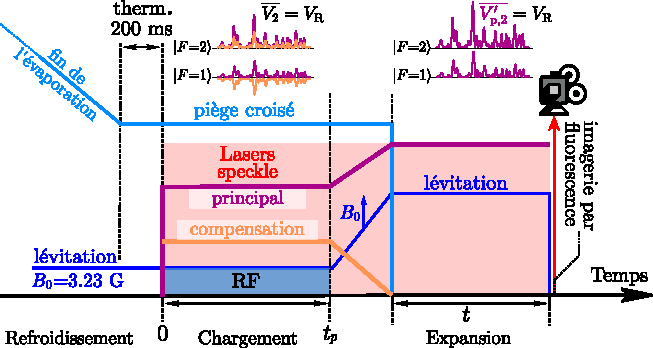
\includegraphics[width=0.9\textwidth]{Fig/Speckle/sequence_spectro_transition.pdf}
\caption{ \textbf{Séquence expérimentale d'étude de la transition d'Anderson.} Après refroidissement et obtention d'un condensat de Bose-Einstein, une étape de chargement du désordre bichromatique (ici représenté répulsif) à énergie résolue est réalisée à l'aide d'un transfert radio-fréquence. Une fois le transfert réalisé, le laser de compensation est éteint afin de maximiser le temps de vie des atomes dans l'état $\protect\etatF{2}{}$. Simultanément, la puissance du laser principal est modifiée afin de garder l'amplitude du potentiel $\overline{V_2}$ constante. Enfin, le piège optique croisé est relâché afin de procéder à l'expansion du nuage dans le désordre, ce qui constitue l'expérience de localisation d'Anderson à proprement parler.}
\label{fig:sequence_spectro_transition}
\end{figure}




\subsection{Étude de la similitude de deux \speckles}
Nous avons ainsi montré que l'utilisation d'un \speckle\ bichromatique permettait d'étendre l'applicabilité du désordre dépendant de l'état interne à l'étude de la transition d'Anderson grâce à l'augmentation du temps de vie des atomes dans le désordre de plus de trois ordres de grandeurs.

Cependant, cette approche repose sur une hypothèse cruciale jusqu'à présent passée sous silence. L'approche de l'utilisation d'une seconde fréquence optique afin de compenser le potentiel ressenti par l'état $\etatF{1}{}$ n'est valable que si nous pouvons compenser le potentiel du laser principal en chaque point de l'espace. Il est donc nécessaire que les variations spatiales du profil d'intensité lumineuse du \speckle\ de compensation soient exactement celles du \speckle\ principal (voir figure \ref{fig:speckle_bichromatique_spatial}):
\begin{equation}
V_{\mathrm{c,1}}(\mathbf{x})=-V_{\mathrm{p,1}}(\mathbf{x}) \text{ .}
\end{equation}

L'étude de la similitude de deux figures de \speckle\ présentée dans cette section représente ma contribution au développement du désordre bichromatique, entamé par Vincent Denechaud et Musawwadah Mukhtar avec le calcul de la polarisatibilité atomique.

\begin{figure}
\centering
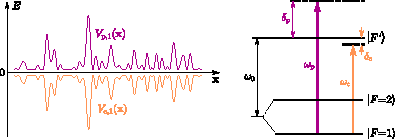
\includegraphics[width=0.9\textwidth]{Fig/Speckle/speckle_bichromatique_spatial.pdf}
\caption{\textbf{Similitude des potentiels générés par chaque laser sur l'état $\mathbf{\protect\etat{F=1}}$.} Afin que le potentiel total ressenti par l'état $\protect\etat{F=1}$ soit nul en tout point de l'espace, il est nécessaire que les potentiels générés par les lasers principal et de compensation soit opposés, c'est à dire $V_{\mathrm{c,1}}(\mathbf{x})=-V_{\mathrm{p,1}}(\mathbf{x})$. Cela implique que le \speckle\ de compensation doit être identique au \speckle\ principal.}
\label{fig:speckle_bichromatique_spatial}
\end{figure}


\paragraph*{Statistique du potentiel total sur $\mathbf{\etatF{1}{}}$}
Étant donné que les degrés de libertés expérimentaux sont déterminés par la condition \ref{eq:contraintes_potentiel_bichromatique}, le potentiel total $V_1(\mathbf{x})=V_{\mathrm{p,1}}(\mathbf{x})+V_{\mathrm{c,1}}(\mathbf{x})$ est de moyenne nulle $\overline{V_1(\mathbf{x})}=0$ par construction. Cependant, sa variance $\sigma_{\mathrm{V}_1}^2(\mathbf{x})$, caractérisant les fluctuations statistiques du potentiel total autour de sa valeur moyenne en un point donné, ne s'annule pas forcément.

%À l'aide des propriétés statistiques des potentiels de type speckle, on montre alors que la variance du potentiel total peut se mettre sous la forme:
%\begin{equation}
%\sigma_{\mathrm{V}_1}^2(\mathbf{x},\lambda_{\mathrm{p}},\lambda_{\mathrm{c}})=2 \left| \overline{V_{\mathrm{p,1}}}(\mathbf{x})\overline{V_{\mathrm{c,1}}}(\mathbf{x})\right| (1+c_{2\lambda}(\mathbf{x})) \quad \text{avec} \quad c_{2\lambda}(\mathbf{x})=\frac{\overline{\delta V_{\mathrm{p,1}}(\mathbf{x}) \delta V_{\mathrm{c,1}}(\mathbf{x})}}{\left|\overline{V_{\mathrm{p,1}}}(\mathbf{x})\overline{V_{\mathrm{c,1}}}(\mathbf{x})\right|} \text{ ,}
%\end{equation}
%en faisant apparaître les fluctuations de potentiel $\delta V_{\mathrm{p,1}}= V_{\mathrm{p,1}}-\overline{V_{\mathrm{p,1}}}$ et $\delta V_{\mathrm{c,1}} = V_{\mathrm{c,1}} - \overline{V_{\mathrm{c,1}}}$. 

Simplifions l'étude en remplaçant les potentiels $V_{\mathrm{p,1}}(\mathbf{x})$ et $V_{\mathrm{c,1}}(\mathbf{x})$ par leurs intensités respectives $I_{\mathrm{p}}(\mathbf{x})$ et $I_{\mathrm{c}}(\mathbf{x})$ de telle sorte que
\begin{equation}
V_1(\mathbf{x})\propto I_{\mathrm{p}}(\mathbf{x}) - I_{\mathrm{c}}(\mathbf{x}) \text{ ,}
\end{equation}
et que $\overline{I_{\mathrm{p}}(\mathbf{x})}=\overline{I_{\mathrm{c}}(\mathbf{x})}=I_0(\mathbf{x})$\footnote{En réalité, les intensités des deux \speckles\ ne sont pas de mêmes valeurs moyennes, cependant il est possible de se ramener formellement à cette situation en tenant compte du fait que les différents désaccords des faisceaux équilibrent les potentiels associés.}. En définissant la différence de ces intensités par la variable $I=I_{\mathrm{p}}-I_{\mathrm{c}}$, l'étude de la variance du potentiel revient à étudier la quantité
\begin{equation}
\sigma_{\mathrm{I}}^2(\mathbf{x},\lambda_{\mathrm{p}},\lambda_{\mathrm{c}})=2 I_0^2(\mathbf{x}) \left(1- c_{\mathrm{2}\lambda}(\mathbf{x}) \right) \quad \text{avec} \quad c_{\mathrm{2}\lambda}(\mathbf{x})=\frac{\overline{\delta I_{\mathrm{p}}(\mathbf{x})\delta I_{\mathrm{c}}(\mathbf{x})}}{I_0^2(\mathbf{x})} \text{ ,}
\label{eq:variance_intensite_bichromatique}
\end{equation}
en faisant apparaître la fonction de corrélation des fluctuations d'intensité. L'interprétation de cette équation est directe: si les deux intensités sont parfaitement corrélées, celles-ci se compensent exactement et $\sigma_{\mathrm{I}}=0$. Dans le cas où celles-ci sont totalement décorrélées, la variance totale est alors la somme des variances de chaque intensité, comme attendu dans le cas de variables aléatoires indépendantes.











\paragraph*{Cohérence temporelle d'une figure de \speckle\ bichromatique}
De manière générale, un champ de speckle résulte de phénomènes d'interférence, et dépend donc fortement de la longueur d'onde du champ incident. Plus particulièrement, nous avons vu dans les sections \ref{sc:correlation_transverse} et \ref{sc:correlation_longitudinale} que la taille des grains de \speckle\ est donnée par la limite de diffraction du système et dépend donc linéairement de la longueur d'onde. 

On comprend donc que si deux profils d'intensité lumineuse sont semblables au point de focalisation des faisceaux, la superposition des grains de lumière se dégrade en s'éloignant de ce point, comme illustré figure \ref{fig:illustration_correlation_double_speckle}. Cette question de superposition des figures d'interférences de plusieurs fréquences optiques est un problème bien connu en optique: il s'agit ici d'étudier l'influence de la cohérence temporelle sur notre désordre bichromatique. Cette influence est quantifiée par la fonction de corrélation des fluctuations d'intensité que nous avons identifiée équation \ref{eq:variance_intensite_bichromatique}, que l'on peut réécrire 
\begin{equation}
\overline{\delta I_{\mathrm{p}}(\mathbf{x}) \delta I_{\mathrm{c}} (\mathbf{x})} = \left| \overline{E_{\mathrm{p}}(\mathbf{x}) E^*_{\mathrm{c}}(\mathbf{x})} \right|^2 \text{ ,}
\end{equation}
à l'aide du théorème de Wick. Il est alors possible d'interpréter cette dernière comme étant le degré de cohérence temporelle en faisant apparaître la fonction de corrélation en amplitude entre les deux champs évalués au même point. En effet, l'objet de notre étude est de quantifier la mesure dans laquelle les deux motifs de \speckle\ sont similaires en un point donné.


Supposons à présent que les modes de chacun des lasers soient identiques et parfaitement superposés\footnote{On satisfait expérimentalement cette hypothèse en injectant les deux faisceaux dans la même fibre optique, voir figure \ref{fig:montage_speckle_bichromatique}.}, de telle sorte que tous deux soient décrits par le même profil d'intensité $I'_0(\xzero)$ de l'équation \ref{eq:profil_intensite_diffuseur}. De même que dans le cas d'un \speckle\ monochromatique, l'expression de la fonction de corrélation en amplitude $\overline{E_{\mathrm{p}}(\mathbf{x}) E^*_{\mathrm{c}}(\mathbf{x})}$ fait apparaître la fonction de corrélation du diffuseur, définie à l'aide de sa transmission:
\begin{equation}
\Cdiff(\xzero,\xzero',\lambda_{\mathrm{p}},\lambda_{\mathrm{c}})=\overline{\tdiff(\xzero,\lambda_{\mathrm{p}})\tdiff^*(\xzero',\lambda_{\mathrm{c}})} \text{ ,}
\end{equation}
dont l'expression a été généralisée au cas bichromatique qui nous intéresse à présent. 

On montre que dans le cas d'un mélange bichromatique, la fonction de corrélation du diffuseur peut s'écrire (voir annexe \ref{ch:anex_speckle}):
\begin{equation}
\Cdiff(\xzero,\xzero',\lambda_{\mathrm{p}},\lambda_{\mathrm{c}})=\exp{\left( -\frac{{\delta\phi}^2}{2}\right) } \exp{\left( -\frac{\pi^2 \theta_{\mathrm{diff}}^2}{2}\frac{(\xzero - \xzero')^2}{\lambda_{\mathrm{p}} \lambda_{\mathrm{c}}} \right)} \text{ ,}
\end{equation}
où la quantité $\delta\phi=\left| \sigma_{\phi,\mathrm{p}} - \sigma_{\phi,\mathrm{c}} \right|$  correspond à la différence des largeurs des distributions de phases induites par le diffuseur aux deux longueurs d'onde d'intérêt $\lambda_{\mathrm{p}}$ et $\lambda_{\mathrm{c}}$. Cette quantité dépend des paramètres géométriques du diffuseur et vaut $\delta\phi\approx 2\pi (n-1) \sigmae/\lambda_{\mathrm{p}}\mathcal{F}$, avec $\mathcal{F}=\lambda_{\mathrm{p}}/\delta\lambda$ une quantité que l'on appellera \emph{finesse} par la suite, par analogie avec le domaine de l'interférométrie.


À l'aide de calculs semblables à ceux utilisés section \ref{sc:speckle_correlation} pour déterminer les propriétés spatiales d'un \speckle\ monochromatique, on détermine que la fonction de corrélation $c_{2\lambda}(\mathbf{x})$ des fluctuations d'intensité à trois dimensions entre les deux \speckles\ générés par le même diffuseur s'exprime aux alentours du plan de Fourier selon (voir annexe \ref{ch:anex_speckle}):
\begin{align}
\nonumber c_{\mathrm{2}\lambda} (\mathbf{x}_{\perp},\delta z) &=\frac{\overline{\delta I_{\mathrm{p}}(\mathbf{x}_{\perp},\delta z) \delta I_{\mathrm{c}}(\mathbf{x}_{\perp},\delta z)}}{I_0^2(\mathbf{x}_{\perp},\delta z)}\\
&=\exp{\left( -\delta\phi^2 \right)}\times c_{\mathrm{3D}}\left(  \frac{\mathbf{x}_{\perp}}{\mathcal{F}}, \frac{\delta z}{\mathcal{F}} \right) \text{ ,}
\label{eq:correlation_2_lambda}
\end{align}
où $c_{\mathrm{3D}}$ correspond à la fonction de corrélation \ref{eq:correlation_3D_paraxial_effectif} des fluctuations d'intensité d'un \speckle\ unique aux alentours du plan de Fourier. 

\begin{figure}
\centering
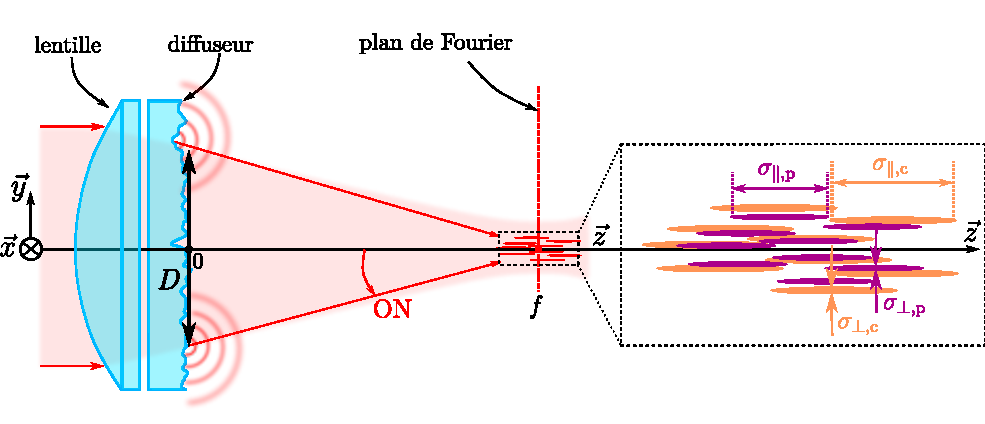
\includegraphics[width=\textwidth]{Fig/Speckle/illustration_correlation_double_speckle.pdf}
\caption{\textbf{Illustration de la cohérence temporelle d'une figure de \speckle .} La taille des grains de \speckle\ dépendant linéairement de la longueur d'onde, ceux-ci ne pourront se superposer que sur une zone restreinte de l'espace. La distance $l_{\mathrm{c}}$ sur laquelle les grains sont corrélés est obtenue à l'aide du degré de cohérence temporelle, et peut être estimée à quelques millimètres.}
\label{fig:illustration_correlation_double_speckle}
\end{figure}

La décorrélation des deux champs vis-à-vis de la cohérence temporelle est donc due à deux contributions:
\begin{itemize}
\item[\textendash] Le premier terme en $\exp{(-\delta\phi^2)}$ décrit l'effet de la propagation dans le diffuseur. Le déphasage accumulé localement dépendant de la longueur d'onde, la distribution de phases diffère entre le laser principal et celui de compensation. Le diffuseur ne se comportant pas exactement de la même manière en fonction de la fréquence de l'onde laser (la transmission $\tdiff(\xzero,\lambda)$ dépend de la longueur d'onde), il en résulte une décorrélation générale entre les profils d'intensité de deux \speckles .
\item[\textendash] Le second terme traduit le déphasage accumulé lors de la propagation du laser, et décrit l'effet de la longueur d'onde du laser sur la taille des grains. Celle-ci étant proportionnelle à la longueur d'onde, les grains des deux figures de \speckle\ seront donc de tailles différentes et ne pourront se superposer que dans une zone réduite de l'espace autour du point de focalisation, comme illustré figure \ref{fig:illustration_correlation_double_speckle}.
\end{itemize}
Une conséquence remarquable de l'équation \ref{eq:correlation_2_lambda} est que la forme de cette fonction, donnée par le degré de cohérence temporelle, est identique à celle de la corrélation spatiale d'un unique \speckle , donnée par le degré de cohérence spatiale. 


La présence du facteur d'échelle $\mathcal{F}=\lambda_{\mathrm{p}}/\delta \lambda$ s'interprète néanmoins aisément. En effet, la taille $\sigma$\footnote{Il n'est pas nécessaire de tenir compte de l'anisotropie des grains de \speckle\ pour ce raisonnement, les longueurs de corrélation transverse et longitudinale étant toutes deux proportionnelles à la longueur d'onde.} d'un grain de \speckle\ est donnée par la largeur de la fonction de corrélation $c_{\mathrm{3D}}$, et est proportionnelle à la longueur d'onde du laser. La largeur de la fonction de corrélation $c_{\mathrm{2}\lambda}$ est donc donnée par la \emph{longueur de cohérence} $l_{\mathrm{c}}=\sigma \mathcal{F}$ et correspond à la distance pour laquelle les grains des deux \speckles\ ne se superposent plus\footnote{Déterminons la distance $L$ sur laquelle deux grains de \speckle\ ne se superposent plus. On définit cette distance comme correspondant à un nombre $N$ de grains du \speckle\ du laser principal $L=N\sigma_{\mathrm{p}}$, et un nombre $N+1$ de grains du laser de compensation $L=(N+1)\sigma_{\mathrm{c}}$. Alors $N=\sigma_{\mathrm{c}}/(\sigma_{\mathrm{p}}-\sigma_{\mathrm{c}})\approx \lambda_{\mathrm{p}}/\delta\lambda=\mathcal{F}$.}.


%En choisissant le désaccord précédent d'environ \SI{100}{\giga\hertz} et une longueur d'onde proche de la transition $D_2$ du \isotope[87]{Rb}, $\lambda_{\mathrm{p}}\approx\SI{780.2}{\nano\metre}$, l'ordre de grandeur de cette longueur de cohérence $l_{\mathrm{c}}$ est donc de plusieurs millimètres. Cette taille étant très grande devant la taille de nos nuages, la décorrélation par décalage des grains des deux \speckles\ ne nous limitera donc pas\footnote{À l'aide d'un banc de test similaire à celui présenté dans la thèse de Jérémie Richard \citep{richard2015propagation}, aucune décorrélation n'a pu être observée expérimentalement dans la limite de résolution du système optique dans une zone de \SI{100}{\micro\metre} autour du centre de la figure de \speckle .}.
Estimons alors l'ordre de grandeur de la longueur de cohérence $l_{\mathrm{c}}$ dans la configuration présentée section \ref{sc:speckle_bichromatique_mukhtar}, pour laquelle la différence de fréquence entre les deux lasers est de l'ordre de \SI{100}{\giga\hertz} pour une longueur d'onde proche de \SI{780}{\nano\metre}. La finesse associée est donc d'environ $\mathcal{F}\approx 4000$. On en déduit que la longueur de cohérence du potentiel bichromatique est de l'ordre de quelques millimètres, c'est-à-dire bien supérieure à la taille de nos nuages. La décorrélation du potentiel par non-superposition des grains ne sera donc pas un facteur limitant pour notre expérience\footnote{À l'aide d'un banc de test similaire à celui présenté dans la thèse de Jérémie Richard \citep{richard2015propagation}, aucune décorrélation n'a pu être observée expérimentalement dans la limite de résolution du système optique dans une zone de \SI{100}{\micro\metre} autour du centre de la figure de \speckle .}.




\paragraph*{Estimation du potentiel résiduel sur $\mathbf{\etatF{1}{}}$}
Si les profils d'intensité des \speckles\ varient de manières similaires à l'échelle des atomes, ceux-ci ne sont pas totalement corrélés, comme le montre le facteur $\exp{( -\delta\phi^2 )}$ de l'équation \ref{eq:correlation_2_lambda}. Ainsi, cela signifie que le potentiel généré par le laser de compensation ne peut annuler le potentiel généré par le laser principal \emph{qu'en moyenne}. Le potentiel total $V_1(\mathbf{x})=V_{\mathrm{p,1}}(\mathbf{x})+V_{\mathrm{c,1}}(\mathbf{x})$ est donc de moyenne nulle $\overline{V_1(\mathbf{x})}=0$ et possède une variance $\sigma_{\mathrm{V}}^2$ non nulle.




Comme nous l'avons vu dans le paragraphe précédent, la variance du potentiel possède une dépendance spatiale correspondant à celle de la fonction de corrélation \ref{eq:correlation_2_lambda}, dont l'échelle de variation est donnée par la longueur de cohérence $l_{\mathrm{c}}$ très grande devant la taille de nos nuages. Il est possible de déterminer la variance du potentiel à l'aide de la valeur au centre de la fonction de corrélation, $c_{\mathrm{2}\lambda}(0)=\exp{(-\delta\phi^2)}$. On peut alors estimer les variations statistiques du potentiel ressenti par les atomes à $\left|\sigma_{\mathrm{V}}/\overline{V_{\mathrm{p,1}}}\right|=\sqrt{\sigma_{\mathrm{I}}^2/I_0^2}$, soit
\begin{equation}
\sigma_{\mathrm{V}}\sim \sqrt{2} \left|\overline{V_{\mathrm{p,1}}} \delta\phi \right| \text{ .}
\end{equation}
Il apparaît donc que l'ordre de grandeur des fluctuations du potentiel bichromatique ne sont qu'une fraction du potentiel généré par chaque laser. 

En supposant que l'épaisseur typique de la granularité du diffuseur $\sigmae$ est de l'ordre de quelques longueurs d'onde $\lambda_{\mathrm{p}}$\footnote{Nous ne possédons malheureusement pas données précises relatives à l'état de surface du diffuseur, il ne s'agit donc que d'une estimation dont l'ordre semble raisonnable. En effet, l'utilisation d'un diffuseur avec $\sigmae\approx 5\lambda_{\mathrm{p}}$ suffit à générer un \speckle\ pleinement développé, la partie déterministe étant très fortement atténuée ($\overline{\tdiff}\sim e^{-100}$).}, on estime ainsi que les fluctuations du potentiel résiduel sont de l'ordre de 
\begin{equation}
\sigma_{\mathrm{V}}\sim 0.01 \overline{V_{\mathrm{p,1}}} \text{ ,}
\end{equation}
avec les paramètres de la configuration précédemment présentée.

De même que dans la section \ref{sc:state_dependent_disorder}, le désordre résiduel que ressent l'état $\etatF{1}{}$ possède une borne supérieure pour laquelle le condensat devient perturbé, finalement du même ordre de grandeur que pour la configuration monochromatique (désordre résiduel de l'ordre de $1\%$ du potentiel appliqué). Ainsi, si les fluctuations du potentiel résiduel sont de l'ordre du potentiel chimique $\mu=\SI{40}{\hertz}$, les modulations de densité ne pourront plus écranter le potentiel désordonné. La condition $\sigma_{\mathrm{V}}\lesssim\mu$ se traduit donc en terme de potentiel maximal applicable aux atomes\footnote{$\VR$ et $\overline{V_{\mathrm{p,1}}}$ ne sont pas identiques, mais sont du même ordre de grandeur. La limite que nous présentons ne se veut pas quantitative étant donné que nous ne donnons qu'une estimation de $\sigmae$ et que la condition $\sigma_{\mathrm{V}}\lesssim\mu$ reste phénoménologique.}
\begin{equation}
\VR\lesssim\SI{4}{\kilo\hertz} \text{ ,}
\end{equation}
semblable à la limite observée dans le cas d'un potentiel dépendant de l'état interne réalisé à l'aide d'une unique fréquence optique. Insistons sur le fait que si la limite du désordre applicable est comparable à celle dans le cas d'un potentiel monochromatique, ce nouveau désordre bichromatique permet l'amélioration du temps de vie dans le désordre de trois ordres de grandeurs, et ouvre donc la voie aux expériences d'expansion et à l'étude de la transition d'Anderson.


\paragraph*{Implémentation expérimentale préliminaire}

Comme annoncé section \ref{sc:montage_diffuseur}, la structure du montage optique du \speckle\ bichromatique suit la même philosophie que les montages présentés précédemment. Dans sa version préliminaire\footnote{À l'heure de l'écriture de ces lignes, seuls des tests préliminaires de stabilité ont pu être effectués. Bien que ceux-ci soient encourageants, il n'est pas exclu que ce montage soit modifié après essai en présence des atomes.}, celui-ci est composé d'un premier étage de mise en forme du faisceau, suivi de la partie générant le \speckle\ rayonné sur les atomes.

\begin{figure}
\centering
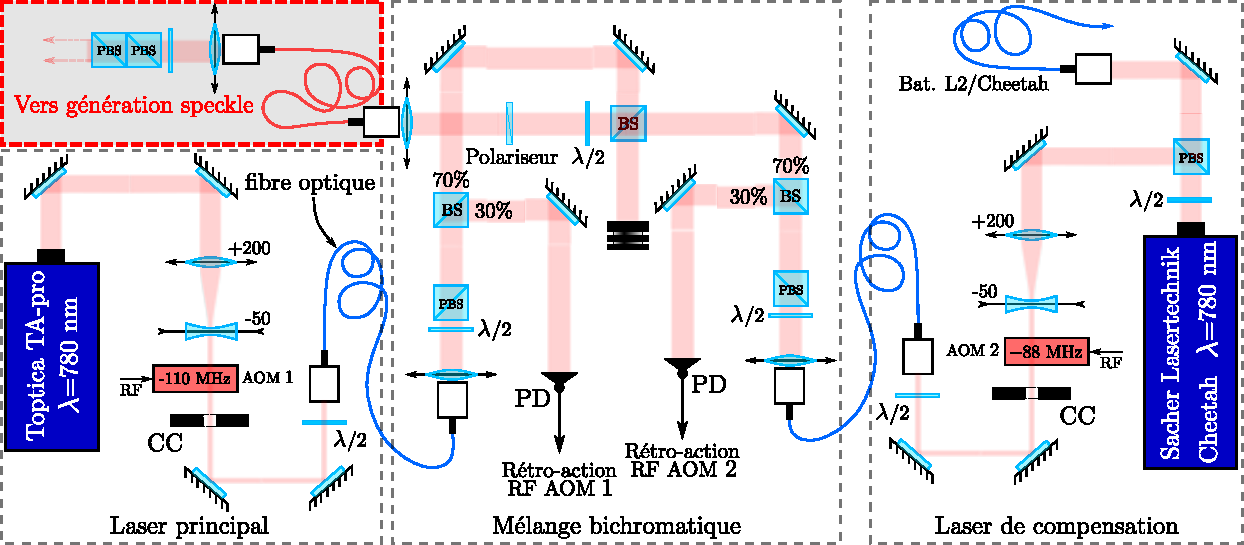
\includegraphics[width=\textwidth]{Fig/Speckle/montage_speckle_bichromatique.pdf}
\caption{\textbf{Montage optique du \speckle\ bichromatique.} De même que pour les montages précédents, le montage optique consiste en une partie de manipulation des faisceaux avant de générer le \speckle . À présent, un étage supplémentaire de mélange des faisceaux est nécessaire, et la présence d'une fibre optique commune assure la parfaite superposition des faisceaux sur le diffuseur.}
\label{fig:montage_speckle_bichromatique}
\end{figure}

Dans le cas de notre nouveau potentiel bichromatique, une étape supplémentaire de superposition des faisceaux est nécessaire afin d'obtenir les mêmes modes laser au niveau du diffuseur. L'ensemble de la partie \emph{mise en forme} est représentée figure \ref{fig:montage_speckle_bichromatique}, et comporte trois zones relatives aux différentes étapes de la mise en forme du faisceau:
\begin{itemize}
\item[\textendash] Une première zone est dédiée à la mise en forme du laser principal et est similaire aux montages précédents. Le faisceau du laser principal est généré par le laser Toptica TA-Pro, et son mode et sa polarisation sont filtrés à l'aide d'une fibre optique à maintien de polarisation et d'un cube séparateur de polarisation. Sa puissance est stabilisée à l'aide d'une boucle de rétroaction réalisée à l'aide d'un modulateur acousto-optique et d'une photodiode, et permet de plus de s'affranchir des fluctuations de puissance liées aux fluctuations de polarisation du laser, comme précédemment. Ce laser étant désaccordé d'environ \SI{100}{\giga\hertz}, il n'est pas nécessaire d'en asservir la fréquence.
\item[\textendash] Une seconde zone, similaire à la première, permet de mettre en forme le faisceau du laser de compensation. Celui-ci est émis par un laser \emph{Sacher Lasertechnik Cheetah} d'une puissance maximale d'environ \SI{100}{\milli\watt}, et subit le même traitement que le faisceau principal. Cependant, la fréquence de ce laser est stabilisée par battement sur le laser repompeur \emph{L2} étant donné son désaccord modéré, de l'ordre de \SI{1.5}{\giga\hertz}.
\item[\textendash] Enfin, une troisième zone permet de combiner dans le même mode spatial les lasers. Pour cela, les faisceaux sont superposés à l'aide d'une lame séparatrice $50/50$, et un polariseur permet de superposer les polarisations des deux lasers. Ceux-ci sont ensuite injectés dans la même fibre optique à maintien de polarisation, garantissant une superposition parfaite des modes pour la génération du \speckle .
\end{itemize}


La partie de génération du \speckle\ est très similaire à celle présentée figure \ref{fig:montage_speckle_specfunc}. La puissance nécessaire sur les atomes étant environ trois ordres de grandeur plus grande que celle utilisée pour la mesure des fonctions spectrales (voir section \ref{sc:state_dependent_disorder} et table \ref{tb:speckle_bichromatique}), la densité optique de transmission $1/1000$ n'est plus nécessaire. Le reste du montage optique est inchangé\footnote{La photodiode précédemment utilisée pour l'asservissement de puissance d'un unique faisceau ne sert plus qu'à titre d'information. En effet, les deux faisceaux étant superposés, il est difficile de les contrôler indépendamment.}.

%\section{Conclusion}
%Dans ce chapitre, nous nous sommes attachés à décrire les propriétés du désordre utilisé sur notre dispositif expérimental. Nous avons ainsi mis en évidence les propriétés statistiques et les propriétés spatiales d'une figure de \speckle , en particulier l'existence d'une longueur de corrélation du champ lumineux se traduit par une taille finie des grains de lumière.

%Dans un second temps, nous avons décrit comment ces propriétés se traduisent en terme de potentiel pour les atomes, pour ensuite discuter de l'approche de désordre dépendant de l'état interne. Les contraintes liées à l'étude de la transition d'Anderson nous ont finalement amenées à envisager la réalisation d'un désordre bichromatique dépendant de l'état interne, dont les performances témoignent d'une forte augmentation du temps de vie des atomes par rapport à la configuration monochromatique, tout en conservant la même limitation sur l'amplitude maximale du désordre.